\section{Synchronisation}\label{SynchronisationTechnique}
\label{Architecture_technique_de_synchronisation}

\subsection{Introduction}
L'objectif de cette section est de décrire les méthodes proposées afin de répondre au problème de synchronisation.
Les échanges de données pouvant être limités (pas de réseau, liaison satellitaire uniquement), il convient de pouvoir choisir précisément les éléments que l'on souhaite synchroniser\footnote{Il est à noter que la synchronisation est bi-directionnelle~: on reçoit les informations du serveur autant qu'on en envoie.}.
\\
Pour permettre la gestion de ces éléments, on introduit la notion de \emph{priorité}~; à chaque catégorie d'éléments (e.g. planning des transports, liste des fournisseurs, informations sur les véhicules, ...) peut être associée une priorité de laquelle dépendra la synchronisation ou non.
À partir de cette \og hiérarchie d'importance \fg{}, on associe des \emph{profils de synchronisation} paramétrables qui -~une fois activés~- gère la synchronisation de façon transparente en fonction des choix de l'utilisateur.
\\
Pour résoudre les problèmes de connexion et assurer le fonctionnement de la suite logicielle indépendamment de la liaison réseau, deux modes sont prévus~:
\begin{itemize}
    \item connecté~;
    \item hors-ligne.
\end{itemize}
L'utilisation de ces deux modes est décrit dans la figure \ref{explicationcodeco}~: on utilise le mode connecté lorsque la liaison réseau est établie avec le serveur local~; et le mode hors-ligne quand il n'y a pas de liaison avec le serveur local.
Dans les deux cas, nous faisons abstraction de la liaison entre le serveur local et le serveur central dans la mesure où l'utilisateur ne se synchronisera qu'avec le serveur local.
% Schéma pour montrer la différence d'utilisation entre le mode connecté et hors ligne :
\begin{figure}[htbp]
    \centering
	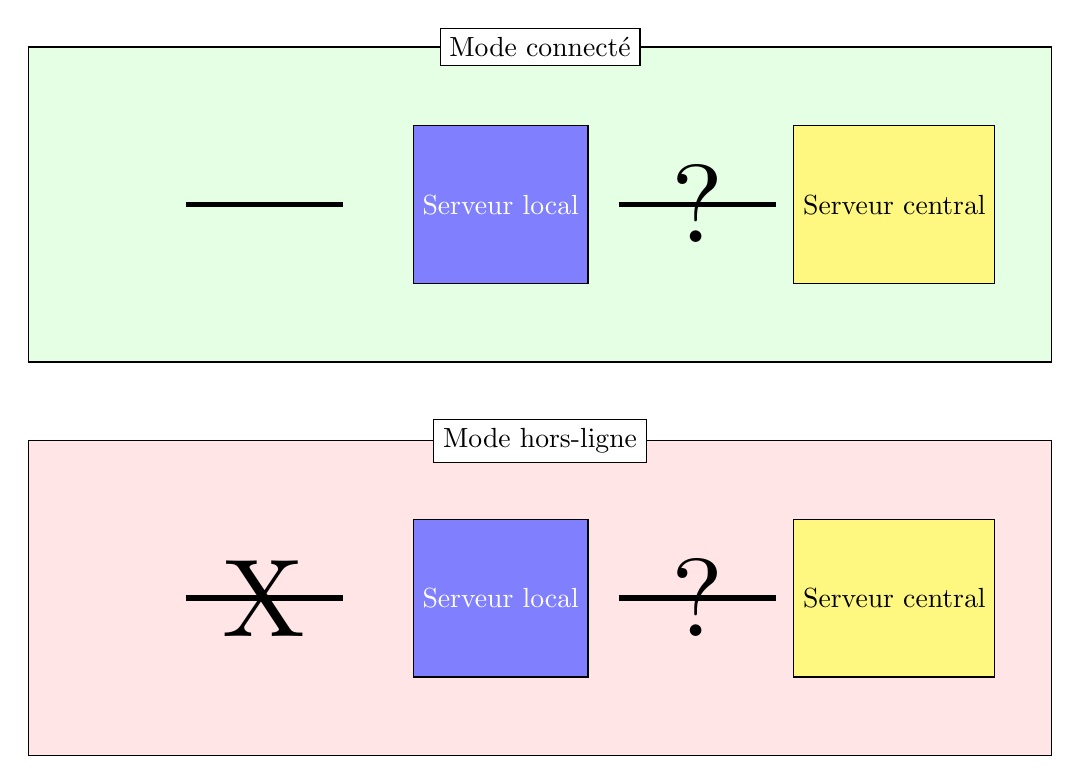
\begin{tikzpicture}
	    % Styles :
		\tikzstyle{titre}=[rectangle,draw,fill=white,text=black]
		\tikzstyle{symbole}=[rectangle,text=black, scale=4]
		\tikzstyle{serveurloc}=[rectangle,draw,fill=blue!50,text=white, minimum height=2cm]
		\tikzstyle{serveurcen}=[rectangle,draw,fill=yellow!50,text=black, minimum height=2cm]
	    % #### CADRE ROUGE :
		% Fond :
		\draw[fill=red!10] (0,0) rectangle (13, 4);
		% Titres :
		\node[titre] at (6.50,4.00) {Mode hors-ligne};
		% Serveurs :
		\node[serveurloc] at (6.00,2) {Serveur local};
		\node[serveurcen] at (11.00,2) {Serveur central};
		\node[symbole] at (8.50,2) {?};
		\node[symbole] at (3.00,2) {X};
		% Traits :
		\draw[line width=2pt] (2, 2) -- (4, 2);
		\draw[line width=2pt] (7.5, 2) -- (9.5, 2);
		% Utilisateurs :
		\umlactor[x=1.00, y=2]{Utilisateur}
		% #### CADRE VERT :
		% Fond :
		\draw[fill=green!10] (0,5) rectangle (13, 9);
		% Titres :
		\node[titre] at (6.50,9.00) {Mode connecté};
		% Serveurs :
		\node[serveurloc] at (6.00,7) {Serveur local};
		\node[serveurcen] at (11.00,7) {Serveur central};
		\node[symbole] at (8.50, 7) {?};
		% Traits :
		\draw[line width=2pt] (2, 7) -- (4, 7);
		\draw[line width=2pt] (7.5, 7) -- (9.5, 7);
		% Utilisateurs :
		\umlactor[x=1.00, y=7]{Utilisateur}
	\end{tikzpicture}
	\caption{Utilisation des modes connecté et hors-ligne}
	\label{explicationcodeco}
\end{figure}

\subsection{Gestion des priorités \& des profils de synchronisation}
Une priorité permet à l'application de \og choisir \fg{} ce qui transite sur le réseau.
Cinq priorités sont définies (par ordre d'importance croissant) pour qualifier des éléments synchronisables~:
\begin{enumerate}
	\item négligeable~;
	\item secondaire~;
	\item normal~;
	\item important~;
	\item crucial.
\end{enumerate}
L'utilisateur peut gérer les priorités à synchroniser en les associant à un profil~: lorsque l'utilisateur choisit un profil de synchronisation, seuls les éléments ayant une priorité inclue dans le profil sont synchronisés.
% Diagramme des CU pour la gestion des profils et des priorités :
\begin{figure}[htbp]
	\centering
	\begin{tikzpicture}
		\begin{umlsystem}[x=8.00,y=5.00,fill=yellow!10]{Priorités des éléments synchronisables}
			\umlusecase[x=0.00,y=1.00,name=MPrio]{Modifier la priorité d'un élément}
		\end{umlsystem}
		\begin{umlsystem}[x=8.00,y=0.00,fill=blue!10]{Profils de synchronisation}
			\umlusecase[x=0.00,y=0.00,name=ChProf]{Choisir un profil}
			\umlusecase[x=0.00,y=1.00,name=EProf]{Éditer un profil}
			\umlusecase[x=0.00,y=2.00,name=CrProf]{Creer un profil}
			\umlusecase[x=0.00,y=3.00,name=SProf]{Supprimer un profil}
		\end{umlsystem}
		\umlactor[x=0.00,y=3.00]{Utilisateur}
		\umlassoc{Utilisateur}{MPrio}
		\umlassoc{Utilisateur}{ChProf}
		\umlassoc{Utilisateur}{EProf}
		\umlassoc{Utilisateur}{CrProf}
		\umlassoc{Utilisateur}{SProf}
	\end{tikzpicture}
	\caption{Diagramme des cas d'utilisation pour la synchronisation}
	\label{ucsynchro}
\end{figure}

\subsection{Mode connecté}
Dans ce mode, on suppose qu'il y a une liaison réseau entre l'utilisateur et le serveur local~; toutes les modifications sont effectuées en \og temps réel\footnote{Un écart de temps pourra être constaté dans le cas où le réseau n'offre qu'un faible débit.} \fg{}.
Pour ce mode, l'utilisateur doit~:
\begin{enumerate}
    \item se connecter~;
    \item utiliser la suite logicielle~;
    \item se déconnecter après utilisation.
\end{enumerate}
L'utilisateur ne pourra effectuer que les modifications dont il a les \emph{permissions}.
% Diagramme des CU pour le mode connecté :
\begin{figure}[htbp]
    \centering
	\begin{tikzpicture}
		\begin{umlsystem}[x=5.00,y=0.00,fill=green!10]{Mode connecté}
			\umlusecase[x=1.00,y=1.50,name=Co]{Se connecter}
			\umlusecase[x=0.00,y=3.00,name=Modif, width=2cm]{Effectuer des modifications}
			\umlusecase[x=6.00,y=1.50,name=ChMode, width=2cm]{Choisir le mode connecté}
			\umlusecase[x=0.00,y=0.00,name=Deco]{Se déconnecter}
		\end{umlsystem}
		\umlactor[x=1.00,y=1.00]{Utilisateur}
		\umlinclude{Co}{ChMode}
		\umlinclude{Deco}{Co} 
		\umlinclude{Modif}{Co} 
		\umlassoc{Utilisateur}{Co}
		\umlassoc{Utilisateur}{Modif}
		\umlassoc{Utilisateur}{Deco}
	\end{tikzpicture}
	\caption{Diagramme des cas d'utilisation pour le mode connecté}
	\label{ucmodeco}
\end{figure}

\subsection{Mode hors-ligne}
Contrairement au mode connecté, le mode hors-ligne permet à l'utilisateur de modifier toutes les informations dont il dispose localement.
Lorsqu'il souhaite synchroniser ses informations avec le serveur, il doit se connecter et c'est à ce moment là que le serveur vérifie que l'utilisateur n'outrepasse pas les droits qui lui sont accordés.
Si c'est le cas, le serveur rejette les modifications locales.
% Diagramme des CU pour le mode hors ligne :
\begin{figure}[htbp]
    \centering
	\begin{tikzpicture}
		\begin{umlsystem}[x=5.00,y=0.00,fill=red!10]{Mode hors-ligne}
			\umlusecase[x=4.50,y=0.20,name=Co]{Se connecter}
			\umlusecase[x=0.00,y=3.00,name=Modif, width=2cm]{Effectuer des modifications}
			\umlusecase[x=6.00,y=3.00,name=ChMode, width=2cm]{Choisir le mode hors-ligne}
			\umlusecase[x=0.00,y=1.00,name=Sync, width=2cm]{Synchroniser avec le serveur}
		\end{umlsystem}
		\umlactor[x=1.00,y=1.00]{Utilisateur}
		\umlinclude{Co}{ChMode}
		\umlinclude{Sync}{Co} 
		\umlassoc{Utilisateur}{Modif}
		\umlassoc{Utilisateur}{Sync}
	\end{tikzpicture}
	\caption{Diagramme des cas d'utilisation pour le mode hors-ligne}
	\label{ucmodedeco}
\end{figure}

\subsection{Gestion des conflits}
Durant la synchronisation, des conflits peuvent survenir au niveau du contenu des informations.
Dans ce cas, l'utilisateur est averti du conflit et des informations qu'il touche et il lui revient le soin de les gérer en choisissant explicitement ce qui est correct et qui doit être enregistré sur le serveur.
\\
Afin de savoir si la version des informations sur le serveur est plus récente (ou plus vieille) que la version locale, un horodatage est mis en place tel que~:
\begin{itemize}
	\item chaque modification locale est horodatée avec l'heure locale~;
	\item à la synchronisation, l'écart temporel entre l'heure locale et l'heure serveur est mesuré\footnote{Par exemple, supposons que la machine locale retarde de deux heures~: si une information a été modifiée à 17h (heure serveur) et qu'une modification est apportée à 16h le même jour en local, l'écart de temps entre les deux machines est mesuré lors de la synchronisation (i.e. deux heures) et permet de dater réellement la modification en local et ainsi déterminer laquelle succède à l'autre.}.
\end{itemize}
Les activités "ajout d'une donnée" (Fig. \ref{SyncAddData}), "modification d'une donnée" (Fig. \ref{SyncModifData}), et "synchronisation" (Fig. \ref{SyncSynchronisation}) représentent les actions réalisées par le programme.

\newpage
\paragraph{Ajout d'une donnée}
\begin{bigcenter}
	\begin{figure}[h]
		\centering
		\scalebox{0.7}{% Graphic for TeX using PGF
% Title: /home/lemon/Bureau/gk/Realisation/Sync_AddData.dia
% Creator: Dia v0.97.2
% CreationDate: Thu Mar 20 21:04:46 2014
% For: lemon
% \usepackage{tikz}
% The following commands are not supported in PSTricks at present
% We define them conditionally, so when they are implemented,
% this pgf file will use them.
\ifx\du\undefined
  \newlength{\du}
\fi
\setlength{\du}{15\unitlength}
\begin{tikzpicture}
\pgftransformxscale{1.000000}
\pgftransformyscale{-1.000000}
\definecolor{dialinecolor}{rgb}{0.000000, 0.000000, 0.000000}
\pgfsetstrokecolor{dialinecolor}
\definecolor{dialinecolor}{rgb}{1.000000, 1.000000, 1.000000}
\pgfsetfillcolor{dialinecolor}
\pgfsetlinewidth{0.100000\du}
\pgfsetdash{}{0pt}
\definecolor{dialinecolor}{rgb}{0.000000, 0.000000, 0.000000}
\pgfsetfillcolor{dialinecolor}
\pgfpathellipse{\pgfpoint{24.289300\du}{1.623090\du}}{\pgfpoint{0.500000\du}{0\du}}{\pgfpoint{0\du}{0.500000\du}}
\pgfusepath{fill}
\pgfsetlinewidth{0.100000\du}
\pgfsetbuttcap
\pgfsetdash{}{0pt}
{
\definecolor{dialinecolor}{rgb}{0.000000, 0.000000, 0.000000}
\pgfsetfillcolor{dialinecolor}
% was here!!!
\pgfsetarrowsend{to}
\definecolor{dialinecolor}{rgb}{0.000000, 0.000000, 0.000000}
\pgfsetstrokecolor{dialinecolor}
\draw (24.289300\du,7.047170\du)--(24.289300\du,7.547170\du)--(24.289300\du,8.607300\du)--(24.289300\du,9.107300\du);
}
% setfont left to latex
\pgfsetlinewidth{0.100000\du}
\pgfsetbuttcap
\pgfsetdash{}{0pt}
{
\definecolor{dialinecolor}{rgb}{0.000000, 0.000000, 0.000000}
\pgfsetfillcolor{dialinecolor}
% was here!!!
\pgfsetarrowsend{to}
\definecolor{dialinecolor}{rgb}{0.000000, 0.000000, 0.000000}
\pgfsetstrokecolor{dialinecolor}
\draw (29.699350\du,36.569400\du)--(29.699350\du,39.001900\du)--(27.651800\du,39.001900\du);
}
% setfont left to latex
\pgfsetlinewidth{0.100000\du}
\pgfsetdash{}{0pt}
{\pgfsetcornersarced{\pgfpoint{1.000000\du}{1.000000\du}}\definecolor{dialinecolor}{rgb}{1.000000, 1.000000, 1.000000}
\pgfsetfillcolor{dialinecolor}
\fill (20.956800\du,37.701900\du)--(20.956800\du,40.301900\du)--(27.651800\du,40.301900\du)--(27.651800\du,37.701900\du)--cycle;
}{\pgfsetcornersarced{\pgfpoint{1.000000\du}{1.000000\du}}\definecolor{dialinecolor}{rgb}{0.000000, 0.000000, 0.000000}
\pgfsetstrokecolor{dialinecolor}
\draw (20.956800\du,37.701900\du)--(20.956800\du,40.301900\du)--(27.651800\du,40.301900\du)--(27.651800\du,37.701900\du)--cycle;
}% setfont left to latex
\definecolor{dialinecolor}{rgb}{0.000000, 0.000000, 0.000000}
\pgfsetstrokecolor{dialinecolor}
\node at (24.304300\du,38.796900\du){Ajouter la donnée};
% setfont left to latex
\definecolor{dialinecolor}{rgb}{0.000000, 0.000000, 0.000000}
\pgfsetstrokecolor{dialinecolor}
\node at (24.304300\du,39.596900\du){en local};
\pgfsetlinewidth{0.100000\du}
\pgfsetdash{}{0pt}
{\pgfsetcornersarced{\pgfpoint{1.000000\du}{1.000000\du}}\definecolor{dialinecolor}{rgb}{1.000000, 1.000000, 1.000000}
\pgfsetfillcolor{dialinecolor}
\fill (21.594300\du,4.447170\du)--(21.594300\du,7.047170\du)--(26.984300\du,7.047170\du)--(26.984300\du,4.447170\du)--cycle;
}{\pgfsetcornersarced{\pgfpoint{1.000000\du}{1.000000\du}}\definecolor{dialinecolor}{rgb}{0.000000, 0.000000, 0.000000}
\pgfsetstrokecolor{dialinecolor}
\draw (21.594300\du,4.447170\du)--(21.594300\du,7.047170\du)--(26.984300\du,7.047170\du)--(26.984300\du,4.447170\du)--cycle;
}% setfont left to latex
\definecolor{dialinecolor}{rgb}{0.000000, 0.000000, 0.000000}
\pgfsetstrokecolor{dialinecolor}
\node at (24.289300\du,5.542170\du){Ajout};
% setfont left to latex
\definecolor{dialinecolor}{rgb}{0.000000, 0.000000, 0.000000}
\pgfsetstrokecolor{dialinecolor}
\node at (24.289300\du,6.342170\du){d'une donnée};
\pgfsetlinewidth{0.100000\du}
\pgfsetbuttcap
\pgfsetdash{}{0pt}
{
\definecolor{dialinecolor}{rgb}{0.000000, 0.000000, 0.000000}
\pgfsetfillcolor{dialinecolor}
% was here!!!
\pgfsetarrowsend{to}
\definecolor{dialinecolor}{rgb}{0.000000, 0.000000, 0.000000}
\pgfsetstrokecolor{dialinecolor}
\draw (24.289300\du,2.173359\du)--(24.289300\du,2.673359\du)--(24.289300\du,3.947170\du)--(24.289300\du,4.447170\du);
}
% setfont left to latex
\pgfsetlinewidth{0.100000\du}
\pgfsetdash{}{0pt}
\definecolor{dialinecolor}{rgb}{1.000000, 1.000000, 1.000000}
\pgfsetfillcolor{dialinecolor}
\fill (23.289300\du,10.107300\du)--(24.289300\du,9.107300\du)--(25.289300\du,10.107300\du)--(24.289300\du,11.107300\du)--cycle;
\definecolor{dialinecolor}{rgb}{0.000000, 0.000000, 0.000000}
\pgfsetstrokecolor{dialinecolor}
\draw (23.289300\du,10.107300\du)--(24.289300\du,9.107300\du)--(25.289300\du,10.107300\du)--(24.289300\du,11.107300\du)--cycle;
% setfont left to latex
\definecolor{dialinecolor}{rgb}{0.000000, 0.000000, 0.000000}
\pgfsetstrokecolor{dialinecolor}
\node[anchor=west] at (25.104500\du,11.972300\du){\ensuremath{[}OUI\ensuremath{]}};
% setfont left to latex
\definecolor{dialinecolor}{rgb}{0.000000, 0.000000, 0.000000}
\pgfsetstrokecolor{dialinecolor}
\node[anchor=west] at (25.276100\du,9.346400\du){\ensuremath{[}NON\ensuremath{]}};
\pgfsetlinewidth{0.100000\du}
\pgfsetbuttcap
\pgfsetdash{}{0pt}
{
\definecolor{dialinecolor}{rgb}{0.000000, 0.000000, 0.000000}
\pgfsetfillcolor{dialinecolor}
% was here!!!
\pgfsetarrowsend{to}
\definecolor{dialinecolor}{rgb}{0.000000, 0.000000, 0.000000}
\pgfsetstrokecolor{dialinecolor}
\draw (24.289300\du,11.107300\du)--(24.289300\du,12.251950\du)--(24.304250\du,12.251950\du)--(24.304250\du,13.396600\du);
}
% setfont left to latex
\pgfsetlinewidth{0.100000\du}
\pgfsetdash{}{0pt}
\definecolor{dialinecolor}{rgb}{1.000000, 1.000000, 1.000000}
\pgfsetfillcolor{dialinecolor}
\fill (23.289300\du,19.134600\du)--(24.289300\du,18.134600\du)--(25.289300\du,19.134600\du)--(24.289300\du,20.134600\du)--cycle;
\definecolor{dialinecolor}{rgb}{0.000000, 0.000000, 0.000000}
\pgfsetstrokecolor{dialinecolor}
\draw (23.289300\du,19.134600\du)--(24.289300\du,18.134600\du)--(25.289300\du,19.134600\du)--(24.289300\du,20.134600\du)--cycle;
% setfont left to latex
\definecolor{dialinecolor}{rgb}{0.000000, 0.000000, 0.000000}
\pgfsetstrokecolor{dialinecolor}
\node[anchor=west] at (25.517000\du,18.868200\du){L'utilisateur a le droit};
% setfont left to latex
\definecolor{dialinecolor}{rgb}{0.000000, 0.000000, 0.000000}
\pgfsetstrokecolor{dialinecolor}
\node[anchor=west] at (25.517000\du,19.668200\du){d'ajouter la donnée};
\pgfsetlinewidth{0.100000\du}
\pgfsetdash{}{0pt}
{\pgfsetcornersarced{\pgfpoint{1.000000\du}{1.000000\du}}\definecolor{dialinecolor}{rgb}{1.000000, 1.000000, 1.000000}
\pgfsetfillcolor{dialinecolor}
\fill (20.533100\du,22.315300\du)--(20.533100\du,24.915300\du)--(28.000600\du,24.915300\du)--(28.000600\du,22.315300\du)--cycle;
}{\pgfsetcornersarced{\pgfpoint{1.000000\du}{1.000000\du}}\definecolor{dialinecolor}{rgb}{0.000000, 0.000000, 0.000000}
\pgfsetstrokecolor{dialinecolor}
\draw (20.533100\du,22.315300\du)--(20.533100\du,24.915300\du)--(28.000600\du,24.915300\du)--(28.000600\du,22.315300\du)--cycle;
}% setfont left to latex
\definecolor{dialinecolor}{rgb}{0.000000, 0.000000, 0.000000}
\pgfsetstrokecolor{dialinecolor}
\node at (24.266850\du,23.410300\du){Envoi de la nouvelle};
% setfont left to latex
\definecolor{dialinecolor}{rgb}{0.000000, 0.000000, 0.000000}
\pgfsetstrokecolor{dialinecolor}
\node at (24.266850\du,24.210300\du){donnée au serveur};
\pgfsetlinewidth{0.100000\du}
\pgfsetbuttcap
\pgfsetdash{}{0pt}
{
\definecolor{dialinecolor}{rgb}{0.000000, 0.000000, 0.000000}
\pgfsetfillcolor{dialinecolor}
% was here!!!
\pgfsetarrowsend{to}
\definecolor{dialinecolor}{rgb}{0.000000, 0.000000, 0.000000}
\pgfsetstrokecolor{dialinecolor}
\draw (24.289300\du,20.134600\du)--(24.289300\du,21.224950\du)--(24.266850\du,21.224950\du)--(24.266850\du,22.315300\du);
}
% setfont left to latex
% setfont left to latex
\definecolor{dialinecolor}{rgb}{0.000000, 0.000000, 0.000000}
\pgfsetstrokecolor{dialinecolor}
\node[anchor=west] at (24.775300\du,20.795500\du){\ensuremath{[}OUI\ensuremath{]}};
% setfont left to latex
\definecolor{dialinecolor}{rgb}{0.000000, 0.000000, 0.000000}
\pgfsetstrokecolor{dialinecolor}
\node[anchor=west] at (20.690500\du,18.398600\du){\ensuremath{[}NON\ensuremath{]}};
\pgfsetlinewidth{0.100000\du}
\pgfsetbuttcap
\pgfsetdash{}{0pt}
{
\definecolor{dialinecolor}{rgb}{0.000000, 0.000000, 0.000000}
\pgfsetfillcolor{dialinecolor}
% was here!!!
\pgfsetarrowsend{to}
\definecolor{dialinecolor}{rgb}{0.000000, 0.000000, 0.000000}
\pgfsetstrokecolor{dialinecolor}
\draw (23.289300\du,19.134600\du)--(16.543300\du,19.134600\du)--(16.543300\du,22.726300\du);
}
% setfont left to latex
\pgfsetlinewidth{0.100000\du}
\pgfsetdash{}{0pt}
{\pgfsetcornersarced{\pgfpoint{1.000000\du}{1.000000\du}}\definecolor{dialinecolor}{rgb}{1.000000, 1.000000, 1.000000}
\pgfsetfillcolor{dialinecolor}
\fill (13.740800\du,22.726300\du)--(13.740800\du,24.526300\du)--(19.345800\du,24.526300\du)--(19.345800\du,22.726300\du)--cycle;
}{\pgfsetcornersarced{\pgfpoint{1.000000\du}{1.000000\du}}\definecolor{dialinecolor}{rgb}{0.000000, 0.000000, 0.000000}
\pgfsetstrokecolor{dialinecolor}
\draw (13.740800\du,22.726300\du)--(13.740800\du,24.526300\du)--(19.345800\du,24.526300\du)--(19.345800\du,22.726300\du)--cycle;
}% setfont left to latex
\definecolor{dialinecolor}{rgb}{0.000000, 0.000000, 0.000000}
\pgfsetstrokecolor{dialinecolor}
\node at (16.543300\du,23.821300\du){Refuser l'ajout};
\pgfsetlinewidth{0.100000\du}
\pgfsetbuttcap
\pgfsetdash{}{0pt}
{
\definecolor{dialinecolor}{rgb}{0.000000, 0.000000, 0.000000}
\pgfsetfillcolor{dialinecolor}
% was here!!!
\pgfsetarrowsend{to}
\definecolor{dialinecolor}{rgb}{0.000000, 0.000000, 0.000000}
\pgfsetstrokecolor{dialinecolor}
\draw (16.543300\du,24.526300\du)--(16.543300\du,47.149400\du)--(23.545600\du,47.149400\du);
}
% setfont left to latex
\pgfsetlinewidth{0.100000\du}
\pgfsetdash{}{0pt}
{\pgfsetcornersarced{\pgfpoint{0.500000\du}{0.500000\du}}\definecolor{dialinecolor}{rgb}{1.000000, 1.000000, 1.000000}
\pgfsetfillcolor{dialinecolor}
\fill (19.590600\du,27.119400\du)--(19.590600\du,29.719400\du)--(28.988100\du,29.719400\du)--(28.988100\du,27.119400\du)--cycle;
}{\pgfsetcornersarced{\pgfpoint{0.500000\du}{0.500000\du}}\definecolor{dialinecolor}{rgb}{0.000000, 0.000000, 0.000000}
\pgfsetstrokecolor{dialinecolor}
\draw (19.590600\du,27.119400\du)--(19.590600\du,29.719400\du)--(28.988100\du,29.719400\du)--(28.988100\du,27.119400\du)--cycle;
}% setfont left to latex
\definecolor{dialinecolor}{rgb}{0.000000, 0.000000, 0.000000}
\pgfsetstrokecolor{dialinecolor}
\node at (24.289350\du,28.214400\du){Attente de la confirmation};
% setfont left to latex
\definecolor{dialinecolor}{rgb}{0.000000, 0.000000, 0.000000}
\pgfsetstrokecolor{dialinecolor}
\node at (24.289350\du,29.014400\du){du serveur};
\pgfsetlinewidth{0.100000\du}
\pgfsetbuttcap
\pgfsetdash{}{0pt}
{
\definecolor{dialinecolor}{rgb}{0.000000, 0.000000, 0.000000}
\pgfsetfillcolor{dialinecolor}
% was here!!!
\pgfsetarrowsend{to}
\definecolor{dialinecolor}{rgb}{0.000000, 0.000000, 0.000000}
\pgfsetstrokecolor{dialinecolor}
\draw (24.266850\du,24.915300\du)--(24.266850\du,26.017350\du)--(24.289350\du,26.017350\du)--(24.289350\du,27.119400\du);
}
% setfont left to latex
\pgfsetlinewidth{0.100000\du}
\pgfsetdash{}{0pt}
\definecolor{dialinecolor}{rgb}{1.000000, 1.000000, 1.000000}
\pgfsetfillcolor{dialinecolor}
\fill (23.289300\du,32.819400\du)--(24.289300\du,31.819400\du)--(25.289300\du,32.819400\du)--(24.289300\du,33.819400\du)--cycle;
\definecolor{dialinecolor}{rgb}{0.000000, 0.000000, 0.000000}
\pgfsetstrokecolor{dialinecolor}
\draw (23.289300\du,32.819400\du)--(24.289300\du,31.819400\du)--(25.289300\du,32.819400\du)--(24.289300\du,33.819400\du)--cycle;
% setfont left to latex
\definecolor{dialinecolor}{rgb}{0.000000, 0.000000, 0.000000}
\pgfsetstrokecolor{dialinecolor}
\node[anchor=west] at (17.790600\du,32.269400\du){La confirmation};
% setfont left to latex
\definecolor{dialinecolor}{rgb}{0.000000, 0.000000, 0.000000}
\pgfsetstrokecolor{dialinecolor}
\node[anchor=west] at (17.790600\du,33.069400\du){a été reçue};
\pgfsetlinewidth{0.100000\du}
\pgfsetbuttcap
\pgfsetdash{}{0pt}
{
\definecolor{dialinecolor}{rgb}{0.000000, 0.000000, 0.000000}
\pgfsetfillcolor{dialinecolor}
% was here!!!
\pgfsetarrowsend{to}
\definecolor{dialinecolor}{rgb}{0.000000, 0.000000, 0.000000}
\pgfsetstrokecolor{dialinecolor}
\draw (24.289350\du,29.719400\du)--(24.289350\du,30.769400\du)--(24.289300\du,30.769400\du)--(24.289300\du,31.819400\du);
}
% setfont left to latex
\pgfsetlinewidth{0.100000\du}
\pgfsetdash{}{0pt}
{\pgfsetcornersarced{\pgfpoint{1.000000\du}{1.000000\du}}\definecolor{dialinecolor}{rgb}{1.000000, 1.000000, 1.000000}
\pgfsetfillcolor{dialinecolor}
\fill (26.140600\du,33.969400\du)--(26.140600\du,36.569400\du)--(33.258100\du,36.569400\du)--(33.258100\du,33.969400\du)--cycle;
}{\pgfsetcornersarced{\pgfpoint{1.000000\du}{1.000000\du}}\definecolor{dialinecolor}{rgb}{0.000000, 0.000000, 0.000000}
\pgfsetstrokecolor{dialinecolor}
\draw (26.140600\du,33.969400\du)--(26.140600\du,36.569400\du)--(33.258100\du,36.569400\du)--(33.258100\du,33.969400\du)--cycle;
}% setfont left to latex
\definecolor{dialinecolor}{rgb}{0.000000, 0.000000, 0.000000}
\pgfsetstrokecolor{dialinecolor}
\node at (29.699350\du,35.064400\du){Arvertir de la perte};
% setfont left to latex
\definecolor{dialinecolor}{rgb}{0.000000, 0.000000, 0.000000}
\pgfsetstrokecolor{dialinecolor}
\node at (29.699350\du,35.864400\du){de connexion};
\pgfsetlinewidth{0.100000\du}
\pgfsetbuttcap
\pgfsetdash{}{0pt}
{
\definecolor{dialinecolor}{rgb}{0.000000, 0.000000, 0.000000}
\pgfsetfillcolor{dialinecolor}
% was here!!!
\pgfsetarrowsend{to}
\definecolor{dialinecolor}{rgb}{0.000000, 0.000000, 0.000000}
\pgfsetstrokecolor{dialinecolor}
\draw (25.289300\du,32.819400\du)--(26.789300\du,32.819400\du)--(26.789300\du,32.819400\du)--(29.699300\du,32.819400\du)--(29.699300\du,33.969400\du);
}
% setfont left to latex
% setfont left to latex
\definecolor{dialinecolor}{rgb}{0.000000, 0.000000, 0.000000}
\pgfsetstrokecolor{dialinecolor}
\node[anchor=west] at (24.995600\du,31.844400\du){\ensuremath{[}NON\ensuremath{]}};
% setfont left to latex
\definecolor{dialinecolor}{rgb}{0.000000, 0.000000, 0.000000}
\pgfsetstrokecolor{dialinecolor}
\node[anchor=west] at (21.695600\du,34.644400\du){\ensuremath{[}OUI\ensuremath{]}};
\pgfsetlinewidth{0.100000\du}
\pgfsetbuttcap
\pgfsetdash{}{0pt}
{
\definecolor{dialinecolor}{rgb}{0.000000, 0.000000, 0.000000}
\pgfsetfillcolor{dialinecolor}
% was here!!!
\pgfsetarrowsend{to}
\definecolor{dialinecolor}{rgb}{0.000000, 0.000000, 0.000000}
\pgfsetstrokecolor{dialinecolor}
\draw (24.289300\du,33.819400\du)--(24.289300\du,35.760650\du)--(24.304300\du,35.760650\du)--(24.304300\du,37.701900\du);
}
% setfont left to latex
\pgfsetlinewidth{0.100000\du}
\pgfsetdash{}{0pt}
{\pgfsetcornersarced{\pgfpoint{1.000000\du}{1.000000\du}}\definecolor{dialinecolor}{rgb}{1.000000, 1.000000, 1.000000}
\pgfsetfillcolor{dialinecolor}
\fill (21.645600\du,42.549400\du)--(21.645600\du,44.349400\du)--(26.970600\du,44.349400\du)--(26.970600\du,42.549400\du)--cycle;
}{\pgfsetcornersarced{\pgfpoint{1.000000\du}{1.000000\du}}\definecolor{dialinecolor}{rgb}{0.000000, 0.000000, 0.000000}
\pgfsetstrokecolor{dialinecolor}
\draw (21.645600\du,42.549400\du)--(21.645600\du,44.349400\du)--(26.970600\du,44.349400\du)--(26.970600\du,42.549400\du)--cycle;
}% setfont left to latex
\definecolor{dialinecolor}{rgb}{0.000000, 0.000000, 0.000000}
\pgfsetstrokecolor{dialinecolor}
\node at (24.308100\du,43.644400\du){Log de l'ajout};
\pgfsetlinewidth{0.100000\du}
\pgfsetbuttcap
\pgfsetdash{}{0pt}
{
\definecolor{dialinecolor}{rgb}{0.000000, 0.000000, 0.000000}
\pgfsetfillcolor{dialinecolor}
% was here!!!
\pgfsetarrowsend{to}
\definecolor{dialinecolor}{rgb}{0.000000, 0.000000, 0.000000}
\pgfsetstrokecolor{dialinecolor}
\draw (24.304300\du,40.301900\du)--(24.304300\du,41.425650\du)--(24.308100\du,41.425650\du)--(24.308100\du,42.549400\du);
}
% setfont left to latex
\pgfsetlinewidth{0.100000\du}
\pgfsetbuttcap
\pgfsetdash{}{0pt}
{
\definecolor{dialinecolor}{rgb}{0.000000, 0.000000, 0.000000}
\pgfsetfillcolor{dialinecolor}
% was here!!!
\pgfsetarrowsend{to}
\definecolor{dialinecolor}{rgb}{0.000000, 0.000000, 0.000000}
\pgfsetstrokecolor{dialinecolor}
\draw (25.289300\du,10.107300\du)--(34.190600\du,10.107300\du)--(34.190600\du,39.001900\du)--(27.651800\du,39.001900\du);
}
% setfont left to latex
\pgfsetlinewidth{0.100000\du}
\pgfsetdash{}{0pt}
\definecolor{dialinecolor}{rgb}{1.000000, 1.000000, 1.000000}
\pgfsetfillcolor{dialinecolor}
\pgfpathellipse{\pgfpoint{24.295600\du}{47.149400\du}}{\pgfpoint{0.750000\du}{0\du}}{\pgfpoint{0\du}{0.750000\du}}
\pgfusepath{fill}
\definecolor{dialinecolor}{rgb}{0.000000, 0.000000, 0.000000}
\pgfsetstrokecolor{dialinecolor}
\pgfpathellipse{\pgfpoint{24.295600\du}{47.149400\du}}{\pgfpoint{0.750000\du}{0\du}}{\pgfpoint{0\du}{0.750000\du}}
\pgfusepath{stroke}
\definecolor{dialinecolor}{rgb}{0.000000, 0.000000, 0.000000}
\pgfsetfillcolor{dialinecolor}
\pgfpathellipse{\pgfpoint{24.295600\du}{47.149400\du}}{\pgfpoint{0.500000\du}{0\du}}{\pgfpoint{0\du}{0.500000\du}}
\pgfusepath{fill}
\pgfsetlinewidth{0.100000\du}
\pgfsetbuttcap
\pgfsetdash{}{0pt}
{
\definecolor{dialinecolor}{rgb}{0.000000, 0.000000, 0.000000}
\pgfsetfillcolor{dialinecolor}
% was here!!!
\pgfsetarrowsend{to}
\definecolor{dialinecolor}{rgb}{0.000000, 0.000000, 0.000000}
\pgfsetstrokecolor{dialinecolor}
\draw (24.308100\du,44.349400\du)--(24.308100\du,45.374400\du)--(24.295600\du,45.374400\du)--(24.295600\du,46.399400\du);
}
% setfont left to latex
% setfont left to latex
\definecolor{dialinecolor}{rgb}{0.000000, 0.000000, 0.000000}
\pgfsetstrokecolor{dialinecolor}
\node[anchor=west] at (18.805000\du,9.975000\du){L'utilisateur};
% setfont left to latex
\definecolor{dialinecolor}{rgb}{0.000000, 0.000000, 0.000000}
\pgfsetstrokecolor{dialinecolor}
\node[anchor=west] at (18.805000\du,10.775000\du){est connecté};
\pgfsetlinewidth{0.100000\du}
\pgfsetdash{}{0pt}
{\pgfsetcornersarced{\pgfpoint{0.500000\du}{0.500000\du}}\definecolor{dialinecolor}{rgb}{1.000000, 1.000000, 1.000000}
\pgfsetfillcolor{dialinecolor}
\fill (19.883000\du,13.396600\du)--(19.883000\du,15.996600\du)--(28.725500\du,15.996600\du)--(28.725500\du,13.396600\du)--cycle;
}{\pgfsetcornersarced{\pgfpoint{0.500000\du}{0.500000\du}}\definecolor{dialinecolor}{rgb}{0.000000, 0.000000, 0.000000}
\pgfsetstrokecolor{dialinecolor}
\draw (19.883000\du,13.396600\du)--(19.883000\du,15.996600\du)--(28.725500\du,15.996600\du)--(28.725500\du,13.396600\du)--cycle;
}% setfont left to latex
\definecolor{dialinecolor}{rgb}{0.000000, 0.000000, 0.000000}
\pgfsetstrokecolor{dialinecolor}
\node at (24.304250\du,14.491600\du){Demander la permission};
% setfont left to latex
\definecolor{dialinecolor}{rgb}{0.000000, 0.000000, 0.000000}
\pgfsetstrokecolor{dialinecolor}
\node at (24.304250\du,15.291600\du){dans l'annuaire};
\pgfsetlinewidth{0.100000\du}
\pgfsetbuttcap
\pgfsetdash{}{0pt}
{
\definecolor{dialinecolor}{rgb}{0.000000, 0.000000, 0.000000}
\pgfsetfillcolor{dialinecolor}
% was here!!!
\pgfsetarrowsend{to}
\definecolor{dialinecolor}{rgb}{0.000000, 0.000000, 0.000000}
\pgfsetstrokecolor{dialinecolor}
\draw (24.304250\du,15.996600\du)--(24.304250\du,17.065600\du)--(24.289300\du,17.065600\du)--(24.289300\du,18.134600\du);
}
% setfont left to latex
\end{tikzpicture}
}
		\caption{Diagramme d'activité~: Ajout d'une donnée}
		\label{SyncAddData}
	\end{figure}
\end{bigcenter}

\newpage
\paragraph{Modification d'une donnée}
\begin{bigcenter}
	\begin{figure}[h]
		\centering
		\scalebox{0.7}{% Graphic for TeX using PGF
% Title: /home/lemon/Bureau/gk/Realisation/Sync_ModifData.dia
% Creator: Dia v0.97.2
% CreationDate: Thu Mar 20 21:08:57 2014
% For: lemon
% \usepackage{tikz}
% The following commands are not supported in PSTricks at present
% We define them conditionally, so when they are implemented,
% this pgf file will use them.
\ifx\du\undefined
  \newlength{\du}
\fi
\setlength{\du}{15\unitlength}
\begin{tikzpicture}
\pgftransformxscale{1.000000}
\pgftransformyscale{-1.000000}
\definecolor{dialinecolor}{rgb}{0.000000, 0.000000, 0.000000}
\pgfsetstrokecolor{dialinecolor}
\definecolor{dialinecolor}{rgb}{1.000000, 1.000000, 1.000000}
\pgfsetfillcolor{dialinecolor}
\pgfsetlinewidth{0.100000\du}
\pgfsetdash{}{0pt}
\definecolor{dialinecolor}{rgb}{0.000000, 0.000000, 0.000000}
\pgfsetfillcolor{dialinecolor}
\pgfpathellipse{\pgfpoint{24.289300\du}{1.673090\du}}{\pgfpoint{0.500000\du}{0\du}}{\pgfpoint{0\du}{0.500000\du}}
\pgfusepath{fill}
\pgfsetlinewidth{0.100000\du}
\pgfsetbuttcap
\pgfsetdash{}{0pt}
{
\definecolor{dialinecolor}{rgb}{0.000000, 0.000000, 0.000000}
\pgfsetfillcolor{dialinecolor}
% was here!!!
\pgfsetarrowsend{to}
\definecolor{dialinecolor}{rgb}{0.000000, 0.000000, 0.000000}
\pgfsetstrokecolor{dialinecolor}
\draw (24.289300\du,7.097170\du)--(24.289300\du,7.597170\du)--(24.289300\du,8.657300\du)--(24.289300\du,9.157300\du);
}
% setfont left to latex
\pgfsetlinewidth{0.100000\du}
\pgfsetbuttcap
\pgfsetdash{}{0pt}
{
\definecolor{dialinecolor}{rgb}{0.000000, 0.000000, 0.000000}
\pgfsetfillcolor{dialinecolor}
% was here!!!
\pgfsetarrowsend{to}
\definecolor{dialinecolor}{rgb}{0.000000, 0.000000, 0.000000}
\pgfsetstrokecolor{dialinecolor}
\draw (37.525300\du,33.818200\du)--(37.525300\du,38.551900\du)--(27.771800\du,38.551900\du);
}
% setfont left to latex
\pgfsetlinewidth{0.100000\du}
\pgfsetbuttcap
\pgfsetdash{}{0pt}
{
\definecolor{dialinecolor}{rgb}{0.000000, 0.000000, 0.000000}
\pgfsetfillcolor{dialinecolor}
% was here!!!
\pgfsetarrowsend{to}
\definecolor{dialinecolor}{rgb}{0.000000, 0.000000, 0.000000}
\pgfsetstrokecolor{dialinecolor}
\draw (38.525300\du,32.818200\du)--(41.746550\du,32.818200\du)--(41.746550\du,34.462700\du);
}
% setfont left to latex
\pgfsetlinewidth{0.100000\du}
\pgfsetdash{}{0pt}
{\pgfsetcornersarced{\pgfpoint{1.000000\du}{1.000000\du}}\definecolor{dialinecolor}{rgb}{1.000000, 1.000000, 1.000000}
\pgfsetfillcolor{dialinecolor}
\fill (38.440300\du,34.462700\du)--(38.440300\du,37.062700\du)--(45.052800\du,37.062700\du)--(45.052800\du,34.462700\du)--cycle;
}{\pgfsetcornersarced{\pgfpoint{1.000000\du}{1.000000\du}}\definecolor{dialinecolor}{rgb}{0.000000, 0.000000, 0.000000}
\pgfsetstrokecolor{dialinecolor}
\draw (38.440300\du,34.462700\du)--(38.440300\du,37.062700\du)--(45.052800\du,37.062700\du)--(45.052800\du,34.462700\du)--cycle;
}% setfont left to latex
\definecolor{dialinecolor}{rgb}{0.000000, 0.000000, 0.000000}
\pgfsetstrokecolor{dialinecolor}
\node at (41.746550\du,35.557700\du){Sauvegarde de la};
% setfont left to latex
\definecolor{dialinecolor}{rgb}{0.000000, 0.000000, 0.000000}
\pgfsetstrokecolor{dialinecolor}
\node at (41.746550\du,36.357700\du){donnée originelle};
\pgfsetlinewidth{0.100000\du}
\pgfsetdash{}{0pt}
{\pgfsetcornersarced{\pgfpoint{1.000000\du}{1.000000\du}}\definecolor{dialinecolor}{rgb}{1.000000, 1.000000, 1.000000}
\pgfsetfillcolor{dialinecolor}
\fill (20.806800\du,37.651900\du)--(20.806800\du,39.451900\du)--(27.771800\du,39.451900\du)--(27.771800\du,37.651900\du)--cycle;
}{\pgfsetcornersarced{\pgfpoint{1.000000\du}{1.000000\du}}\definecolor{dialinecolor}{rgb}{0.000000, 0.000000, 0.000000}
\pgfsetstrokecolor{dialinecolor}
\draw (20.806800\du,37.651900\du)--(20.806800\du,39.451900\du)--(27.771800\du,39.451900\du)--(27.771800\du,37.651900\du)--cycle;
}% setfont left to latex
\definecolor{dialinecolor}{rgb}{0.000000, 0.000000, 0.000000}
\pgfsetstrokecolor{dialinecolor}
\node at (24.289300\du,38.746900\du){Modifier la donnée};
\pgfsetlinewidth{0.100000\du}
\pgfsetbuttcap
\pgfsetdash{}{0pt}
{
\definecolor{dialinecolor}{rgb}{0.000000, 0.000000, 0.000000}
\pgfsetfillcolor{dialinecolor}
% was here!!!
\pgfsetarrowsend{to}
\definecolor{dialinecolor}{rgb}{0.000000, 0.000000, 0.000000}
\pgfsetstrokecolor{dialinecolor}
\draw (41.746550\du,37.062700\du)--(41.746550\du,38.562700\du)--(35.009175\du,38.562700\du)--(35.009175\du,38.551900\du)--(27.771800\du,38.551900\du);
}
% setfont left to latex
\pgfsetlinewidth{0.100000\du}
\pgfsetdash{}{0pt}
{\pgfsetcornersarced{\pgfpoint{1.000000\du}{1.000000\du}}\definecolor{dialinecolor}{rgb}{1.000000, 1.000000, 1.000000}
\pgfsetfillcolor{dialinecolor}
\fill (21.594300\du,4.497170\du)--(21.594300\du,7.097170\du)--(26.984300\du,7.097170\du)--(26.984300\du,4.497170\du)--cycle;
}{\pgfsetcornersarced{\pgfpoint{1.000000\du}{1.000000\du}}\definecolor{dialinecolor}{rgb}{0.000000, 0.000000, 0.000000}
\pgfsetstrokecolor{dialinecolor}
\draw (21.594300\du,4.497170\du)--(21.594300\du,7.097170\du)--(26.984300\du,7.097170\du)--(26.984300\du,4.497170\du)--cycle;
}% setfont left to latex
\definecolor{dialinecolor}{rgb}{0.000000, 0.000000, 0.000000}
\pgfsetstrokecolor{dialinecolor}
\node at (24.289300\du,5.592170\du){Modification};
% setfont left to latex
\definecolor{dialinecolor}{rgb}{0.000000, 0.000000, 0.000000}
\pgfsetstrokecolor{dialinecolor}
\node at (24.289300\du,6.392170\du){d'une donnée};
\pgfsetlinewidth{0.100000\du}
\pgfsetdash{}{0pt}
\definecolor{dialinecolor}{rgb}{1.000000, 1.000000, 1.000000}
\pgfsetfillcolor{dialinecolor}
\fill (36.525300\du,32.818200\du)--(37.525300\du,31.818200\du)--(38.525300\du,32.818200\du)--(37.525300\du,33.818200\du)--cycle;
\definecolor{dialinecolor}{rgb}{0.000000, 0.000000, 0.000000}
\pgfsetstrokecolor{dialinecolor}
\draw (36.525300\du,32.818200\du)--(37.525300\du,31.818200\du)--(38.525300\du,32.818200\du)--(37.525300\du,33.818200\du)--cycle;
% setfont left to latex
\definecolor{dialinecolor}{rgb}{0.000000, 0.000000, 0.000000}
\pgfsetstrokecolor{dialinecolor}
\node[anchor=west] at (35.374100\du,34.926500\du){\ensuremath{[}OUI\ensuremath{]}};
% setfont left to latex
\definecolor{dialinecolor}{rgb}{0.000000, 0.000000, 0.000000}
\pgfsetstrokecolor{dialinecolor}
\node[anchor=west] at (38.995600\du,32.100600\du){\ensuremath{[}NON\ensuremath{]}};
% setfont left to latex
\definecolor{dialinecolor}{rgb}{0.000000, 0.000000, 0.000000}
\pgfsetstrokecolor{dialinecolor}
\node[anchor=west] at (38.148200\du,29.813500\du){La donnée a déjà};
% setfont left to latex
\definecolor{dialinecolor}{rgb}{0.000000, 0.000000, 0.000000}
\pgfsetstrokecolor{dialinecolor}
\node[anchor=west] at (38.148200\du,30.613500\du){été modifiée ?};
\pgfsetlinewidth{0.100000\du}
\pgfsetbuttcap
\pgfsetdash{}{0pt}
{
\definecolor{dialinecolor}{rgb}{0.000000, 0.000000, 0.000000}
\pgfsetfillcolor{dialinecolor}
% was here!!!
\pgfsetarrowsend{to}
\definecolor{dialinecolor}{rgb}{0.000000, 0.000000, 0.000000}
\pgfsetstrokecolor{dialinecolor}
\draw (24.289300\du,2.223359\du)--(24.289300\du,2.723359\du)--(24.289300\du,3.997170\du)--(24.289300\du,4.497170\du);
}
% setfont left to latex
\pgfsetlinewidth{0.100000\du}
\pgfsetdash{}{0pt}
\definecolor{dialinecolor}{rgb}{1.000000, 1.000000, 1.000000}
\pgfsetfillcolor{dialinecolor}
\fill (23.289300\du,10.157300\du)--(24.289300\du,9.157300\du)--(25.289300\du,10.157300\du)--(24.289300\du,11.157300\du)--cycle;
\definecolor{dialinecolor}{rgb}{0.000000, 0.000000, 0.000000}
\pgfsetstrokecolor{dialinecolor}
\draw (23.289300\du,10.157300\du)--(24.289300\du,9.157300\du)--(25.289300\du,10.157300\du)--(24.289300\du,11.157300\du)--cycle;
% setfont left to latex
\definecolor{dialinecolor}{rgb}{0.000000, 0.000000, 0.000000}
\pgfsetstrokecolor{dialinecolor}
\node[anchor=west] at (19.072000\du,10.078400\du){L'utilisateur};
% setfont left to latex
\definecolor{dialinecolor}{rgb}{0.000000, 0.000000, 0.000000}
\pgfsetstrokecolor{dialinecolor}
\node[anchor=west] at (19.072000\du,10.878400\du){est connecté};
% setfont left to latex
\definecolor{dialinecolor}{rgb}{0.000000, 0.000000, 0.000000}
\pgfsetstrokecolor{dialinecolor}
\node[anchor=west] at (25.104500\du,12.022300\du){\ensuremath{[}OUI\ensuremath{]}};
% setfont left to latex
\definecolor{dialinecolor}{rgb}{0.000000, 0.000000, 0.000000}
\pgfsetstrokecolor{dialinecolor}
\node[anchor=west] at (25.276100\du,9.396400\du){\ensuremath{[}NON\ensuremath{]}};
\pgfsetlinewidth{0.100000\du}
\pgfsetbuttcap
\pgfsetdash{}{0pt}
{
\definecolor{dialinecolor}{rgb}{0.000000, 0.000000, 0.000000}
\pgfsetfillcolor{dialinecolor}
% was here!!!
\pgfsetarrowsend{to}
\definecolor{dialinecolor}{rgb}{0.000000, 0.000000, 0.000000}
\pgfsetstrokecolor{dialinecolor}
\draw (25.289300\du,10.157300\du)--(25.289300\du,10.150000\du)--(37.525300\du,10.150000\du)--(37.525300\du,31.818200\du);
}
% setfont left to latex
\pgfsetlinewidth{0.100000\du}
\pgfsetbuttcap
\pgfsetdash{}{0pt}
{
\definecolor{dialinecolor}{rgb}{0.000000, 0.000000, 0.000000}
\pgfsetfillcolor{dialinecolor}
% was here!!!
\pgfsetarrowsend{to}
\definecolor{dialinecolor}{rgb}{0.000000, 0.000000, 0.000000}
\pgfsetstrokecolor{dialinecolor}
\draw (24.289300\du,11.157300\du)--(24.289300\du,12.203650\du)--(24.321250\du,12.203650\du)--(24.321250\du,13.250000\du);
}
% setfont left to latex
\pgfsetlinewidth{0.100000\du}
\pgfsetdash{}{0pt}
\definecolor{dialinecolor}{rgb}{1.000000, 1.000000, 1.000000}
\pgfsetfillcolor{dialinecolor}
\fill (23.289300\du,19.134600\du)--(24.289300\du,18.134600\du)--(25.289300\du,19.134600\du)--(24.289300\du,20.134600\du)--cycle;
\definecolor{dialinecolor}{rgb}{0.000000, 0.000000, 0.000000}
\pgfsetstrokecolor{dialinecolor}
\draw (23.289300\du,19.134600\du)--(24.289300\du,18.134600\du)--(25.289300\du,19.134600\du)--(24.289300\du,20.134600\du)--cycle;
% setfont left to latex
\definecolor{dialinecolor}{rgb}{0.000000, 0.000000, 0.000000}
\pgfsetstrokecolor{dialinecolor}
\node[anchor=west] at (25.517000\du,18.868200\du){L'utilisateur a le droit};
% setfont left to latex
\definecolor{dialinecolor}{rgb}{0.000000, 0.000000, 0.000000}
\pgfsetstrokecolor{dialinecolor}
\node[anchor=west] at (25.517000\du,19.668200\du){de modifier la donnée};
\pgfsetlinewidth{0.100000\du}
\pgfsetdash{}{0pt}
{\pgfsetcornersarced{\pgfpoint{1.000000\du}{1.000000\du}}\definecolor{dialinecolor}{rgb}{1.000000, 1.000000, 1.000000}
\pgfsetfillcolor{dialinecolor}
\fill (19.933100\du,22.315300\du)--(19.933100\du,24.915300\du)--(28.645600\du,24.915300\du)--(28.645600\du,22.315300\du)--cycle;
}{\pgfsetcornersarced{\pgfpoint{1.000000\du}{1.000000\du}}\definecolor{dialinecolor}{rgb}{0.000000, 0.000000, 0.000000}
\pgfsetstrokecolor{dialinecolor}
\draw (19.933100\du,22.315300\du)--(19.933100\du,24.915300\du)--(28.645600\du,24.915300\du)--(28.645600\du,22.315300\du)--cycle;
}% setfont left to latex
\definecolor{dialinecolor}{rgb}{0.000000, 0.000000, 0.000000}
\pgfsetstrokecolor{dialinecolor}
\node at (24.289350\du,23.410300\du){Envoi de la modification};
% setfont left to latex
\definecolor{dialinecolor}{rgb}{0.000000, 0.000000, 0.000000}
\pgfsetstrokecolor{dialinecolor}
\node at (24.289350\du,24.210300\du){au serveur};
\pgfsetlinewidth{0.100000\du}
\pgfsetbuttcap
\pgfsetdash{}{0pt}
{
\definecolor{dialinecolor}{rgb}{0.000000, 0.000000, 0.000000}
\pgfsetfillcolor{dialinecolor}
% was here!!!
\pgfsetarrowsend{to}
\definecolor{dialinecolor}{rgb}{0.000000, 0.000000, 0.000000}
\pgfsetstrokecolor{dialinecolor}
\draw (24.289300\du,20.134600\du)--(24.289300\du,21.224950\du)--(24.289350\du,21.224950\du)--(24.289350\du,22.315300\du);
}
% setfont left to latex
% setfont left to latex
\definecolor{dialinecolor}{rgb}{0.000000, 0.000000, 0.000000}
\pgfsetstrokecolor{dialinecolor}
\node[anchor=west] at (24.775300\du,20.795500\du){\ensuremath{[}OUI\ensuremath{]}};
% setfont left to latex
\definecolor{dialinecolor}{rgb}{0.000000, 0.000000, 0.000000}
\pgfsetstrokecolor{dialinecolor}
\node[anchor=west] at (20.690500\du,18.398600\du){\ensuremath{[}NON\ensuremath{]}};
\pgfsetlinewidth{0.100000\du}
\pgfsetbuttcap
\pgfsetdash{}{0pt}
{
\definecolor{dialinecolor}{rgb}{0.000000, 0.000000, 0.000000}
\pgfsetfillcolor{dialinecolor}
% was here!!!
\pgfsetarrowsend{to}
\definecolor{dialinecolor}{rgb}{0.000000, 0.000000, 0.000000}
\pgfsetstrokecolor{dialinecolor}
\draw (23.289300\du,19.134600\du)--(15.827050\du,19.134600\du)--(15.827050\du,22.526300\du);
}
% setfont left to latex
\pgfsetlinewidth{0.100000\du}
\pgfsetdash{}{0pt}
{\pgfsetcornersarced{\pgfpoint{1.000000\du}{1.000000\du}}\definecolor{dialinecolor}{rgb}{1.000000, 1.000000, 1.000000}
\pgfsetfillcolor{dialinecolor}
\fill (13.340800\du,22.526300\du)--(13.340800\du,25.126300\du)--(18.313300\du,25.126300\du)--(18.313300\du,22.526300\du)--cycle;
}{\pgfsetcornersarced{\pgfpoint{1.000000\du}{1.000000\du}}\definecolor{dialinecolor}{rgb}{0.000000, 0.000000, 0.000000}
\pgfsetstrokecolor{dialinecolor}
\draw (13.340800\du,22.526300\du)--(13.340800\du,25.126300\du)--(18.313300\du,25.126300\du)--(18.313300\du,22.526300\du)--cycle;
}% setfont left to latex
\definecolor{dialinecolor}{rgb}{0.000000, 0.000000, 0.000000}
\pgfsetstrokecolor{dialinecolor}
\node at (15.827050\du,23.621300\du){Refuser la};
% setfont left to latex
\definecolor{dialinecolor}{rgb}{0.000000, 0.000000, 0.000000}
\pgfsetstrokecolor{dialinecolor}
\node at (15.827050\du,24.421300\du){modification};
\pgfsetlinewidth{0.100000\du}
\pgfsetdash{}{0pt}
{\pgfsetcornersarced{\pgfpoint{0.500000\du}{0.500000\du}}\definecolor{dialinecolor}{rgb}{1.000000, 1.000000, 1.000000}
\pgfsetfillcolor{dialinecolor}
\fill (19.590600\du,27.119400\du)--(19.590600\du,29.719400\du)--(28.988100\du,29.719400\du)--(28.988100\du,27.119400\du)--cycle;
}{\pgfsetcornersarced{\pgfpoint{0.500000\du}{0.500000\du}}\definecolor{dialinecolor}{rgb}{0.000000, 0.000000, 0.000000}
\pgfsetstrokecolor{dialinecolor}
\draw (19.590600\du,27.119400\du)--(19.590600\du,29.719400\du)--(28.988100\du,29.719400\du)--(28.988100\du,27.119400\du)--cycle;
}% setfont left to latex
\definecolor{dialinecolor}{rgb}{0.000000, 0.000000, 0.000000}
\pgfsetstrokecolor{dialinecolor}
\node at (24.289350\du,28.214400\du){Attente de la confirmation};
% setfont left to latex
\definecolor{dialinecolor}{rgb}{0.000000, 0.000000, 0.000000}
\pgfsetstrokecolor{dialinecolor}
\node at (24.289350\du,29.014400\du){du serveur};
\pgfsetlinewidth{0.100000\du}
\pgfsetbuttcap
\pgfsetdash{}{0pt}
{
\definecolor{dialinecolor}{rgb}{0.000000, 0.000000, 0.000000}
\pgfsetfillcolor{dialinecolor}
% was here!!!
\pgfsetarrowsend{to}
\definecolor{dialinecolor}{rgb}{0.000000, 0.000000, 0.000000}
\pgfsetstrokecolor{dialinecolor}
\draw (24.289350\du,24.915300\du)--(24.289350\du,25.415300\du)--(24.289350\du,26.619400\du)--(24.289350\du,27.119400\du);
}
% setfont left to latex
\pgfsetlinewidth{0.100000\du}
\pgfsetdash{}{0pt}
\definecolor{dialinecolor}{rgb}{1.000000, 1.000000, 1.000000}
\pgfsetfillcolor{dialinecolor}
\fill (23.289300\du,32.819400\du)--(24.289300\du,31.819400\du)--(25.289300\du,32.819400\du)--(24.289300\du,33.819400\du)--cycle;
\definecolor{dialinecolor}{rgb}{0.000000, 0.000000, 0.000000}
\pgfsetstrokecolor{dialinecolor}
\draw (23.289300\du,32.819400\du)--(24.289300\du,31.819400\du)--(25.289300\du,32.819400\du)--(24.289300\du,33.819400\du)--cycle;
% setfont left to latex
\definecolor{dialinecolor}{rgb}{0.000000, 0.000000, 0.000000}
\pgfsetstrokecolor{dialinecolor}
\node[anchor=west] at (18.140600\du,32.269400\du){La confirmation};
% setfont left to latex
\definecolor{dialinecolor}{rgb}{0.000000, 0.000000, 0.000000}
\pgfsetstrokecolor{dialinecolor}
\node[anchor=west] at (18.140600\du,33.069400\du){a été reçue};
\pgfsetlinewidth{0.100000\du}
\pgfsetbuttcap
\pgfsetdash{}{0pt}
{
\definecolor{dialinecolor}{rgb}{0.000000, 0.000000, 0.000000}
\pgfsetfillcolor{dialinecolor}
% was here!!!
\pgfsetarrowsend{to}
\definecolor{dialinecolor}{rgb}{0.000000, 0.000000, 0.000000}
\pgfsetstrokecolor{dialinecolor}
\draw (24.289350\du,29.719400\du)--(24.289350\du,30.769400\du)--(24.289300\du,30.769400\du)--(24.289300\du,31.819400\du);
}
% setfont left to latex
\pgfsetlinewidth{0.100000\du}
\pgfsetdash{}{0pt}
{\pgfsetcornersarced{\pgfpoint{1.000000\du}{1.000000\du}}\definecolor{dialinecolor}{rgb}{1.000000, 1.000000, 1.000000}
\pgfsetfillcolor{dialinecolor}
\fill (27.340600\du,31.519400\du)--(27.340600\du,34.119400\du)--(34.458100\du,34.119400\du)--(34.458100\du,31.519400\du)--cycle;
}{\pgfsetcornersarced{\pgfpoint{1.000000\du}{1.000000\du}}\definecolor{dialinecolor}{rgb}{0.000000, 0.000000, 0.000000}
\pgfsetstrokecolor{dialinecolor}
\draw (27.340600\du,31.519400\du)--(27.340600\du,34.119400\du)--(34.458100\du,34.119400\du)--(34.458100\du,31.519400\du)--cycle;
}% setfont left to latex
\definecolor{dialinecolor}{rgb}{0.000000, 0.000000, 0.000000}
\pgfsetstrokecolor{dialinecolor}
\node at (30.899350\du,32.614400\du){Arvertir de la perte};
% setfont left to latex
\definecolor{dialinecolor}{rgb}{0.000000, 0.000000, 0.000000}
\pgfsetstrokecolor{dialinecolor}
\node at (30.899350\du,33.414400\du){de connexion};
\pgfsetlinewidth{0.100000\du}
\pgfsetbuttcap
\pgfsetdash{}{0pt}
{
\definecolor{dialinecolor}{rgb}{0.000000, 0.000000, 0.000000}
\pgfsetfillcolor{dialinecolor}
% was here!!!
\pgfsetarrowsend{to}
\definecolor{dialinecolor}{rgb}{0.000000, 0.000000, 0.000000}
\pgfsetstrokecolor{dialinecolor}
\draw (25.289300\du,32.819400\du)--(25.789300\du,32.819400\du)--(26.840600\du,32.819400\du)--(27.340600\du,32.819400\du);
}
% setfont left to latex
% setfont left to latex
\definecolor{dialinecolor}{rgb}{0.000000, 0.000000, 0.000000}
\pgfsetstrokecolor{dialinecolor}
\node[anchor=west] at (24.995600\du,31.844400\du){\ensuremath{[}NON\ensuremath{]}};
% setfont left to latex
\definecolor{dialinecolor}{rgb}{0.000000, 0.000000, 0.000000}
\pgfsetstrokecolor{dialinecolor}
\node[anchor=west] at (21.695600\du,34.644400\du){\ensuremath{[}OUI\ensuremath{]}};
\pgfsetlinewidth{0.100000\du}
\pgfsetbuttcap
\pgfsetdash{}{0pt}
{
\definecolor{dialinecolor}{rgb}{0.000000, 0.000000, 0.000000}
\pgfsetfillcolor{dialinecolor}
% was here!!!
\pgfsetarrowsend{to}
\definecolor{dialinecolor}{rgb}{0.000000, 0.000000, 0.000000}
\pgfsetstrokecolor{dialinecolor}
\draw (34.458100\du,32.819400\du)--(35.491700\du,32.819400\du)--(35.491700\du,32.818200\du)--(36.525300\du,32.818200\du);
}
% setfont left to latex
\pgfsetlinewidth{0.100000\du}
\pgfsetbuttcap
\pgfsetdash{}{0pt}
{
\definecolor{dialinecolor}{rgb}{0.000000, 0.000000, 0.000000}
\pgfsetfillcolor{dialinecolor}
% was here!!!
\pgfsetarrowsend{to}
\definecolor{dialinecolor}{rgb}{0.000000, 0.000000, 0.000000}
\pgfsetstrokecolor{dialinecolor}
\draw (24.289300\du,33.819400\du)--(24.289300\du,34.319400\du)--(24.289300\du,37.151900\du)--(24.289300\du,37.651900\du);
}
% setfont left to latex
\pgfsetlinewidth{0.100000\du}
\pgfsetdash{}{0pt}
{\pgfsetcornersarced{\pgfpoint{1.000000\du}{1.000000\du}}\definecolor{dialinecolor}{rgb}{1.000000, 1.000000, 1.000000}
\pgfsetfillcolor{dialinecolor}
\fill (20.245600\du,41.549400\du)--(20.245600\du,43.349400\du)--(28.345600\du,43.349400\du)--(28.345600\du,41.549400\du)--cycle;
}{\pgfsetcornersarced{\pgfpoint{1.000000\du}{1.000000\du}}\definecolor{dialinecolor}{rgb}{0.000000, 0.000000, 0.000000}
\pgfsetstrokecolor{dialinecolor}
\draw (20.245600\du,41.549400\du)--(20.245600\du,43.349400\du)--(28.345600\du,43.349400\du)--(28.345600\du,41.549400\du)--cycle;
}% setfont left to latex
\definecolor{dialinecolor}{rgb}{0.000000, 0.000000, 0.000000}
\pgfsetstrokecolor{dialinecolor}
\node at (24.295600\du,42.644400\du){Log de la modification};
\pgfsetlinewidth{0.100000\du}
\pgfsetbuttcap
\pgfsetdash{}{0pt}
{
\definecolor{dialinecolor}{rgb}{0.000000, 0.000000, 0.000000}
\pgfsetfillcolor{dialinecolor}
% was here!!!
\pgfsetarrowsend{to}
\definecolor{dialinecolor}{rgb}{0.000000, 0.000000, 0.000000}
\pgfsetstrokecolor{dialinecolor}
\draw (24.289300\du,39.451900\du)--(24.289300\du,40.500650\du)--(24.295600\du,40.500650\du)--(24.295600\du,41.549400\du);
}
% setfont left to latex
\pgfsetlinewidth{0.100000\du}
\pgfsetdash{}{0pt}
\definecolor{dialinecolor}{rgb}{1.000000, 1.000000, 1.000000}
\pgfsetfillcolor{dialinecolor}
\pgfpathellipse{\pgfpoint{24.300000\du}{46.100000\du}}{\pgfpoint{0.750000\du}{0\du}}{\pgfpoint{0\du}{0.750000\du}}
\pgfusepath{fill}
\definecolor{dialinecolor}{rgb}{0.000000, 0.000000, 0.000000}
\pgfsetstrokecolor{dialinecolor}
\pgfpathellipse{\pgfpoint{24.300000\du}{46.100000\du}}{\pgfpoint{0.750000\du}{0\du}}{\pgfpoint{0\du}{0.750000\du}}
\pgfusepath{stroke}
\definecolor{dialinecolor}{rgb}{0.000000, 0.000000, 0.000000}
\pgfsetfillcolor{dialinecolor}
\pgfpathellipse{\pgfpoint{24.300000\du}{46.100000\du}}{\pgfpoint{0.500000\du}{0\du}}{\pgfpoint{0\du}{0.500000\du}}
\pgfusepath{fill}
\pgfsetlinewidth{0.100000\du}
\pgfsetbuttcap
\pgfsetdash{}{0pt}
{
\definecolor{dialinecolor}{rgb}{0.000000, 0.000000, 0.000000}
\pgfsetfillcolor{dialinecolor}
% was here!!!
\pgfsetarrowsend{to}
\definecolor{dialinecolor}{rgb}{0.000000, 0.000000, 0.000000}
\pgfsetstrokecolor{dialinecolor}
\draw (15.827050\du,25.126300\du)--(15.827050\du,46.100000\du)--(23.550000\du,46.100000\du);
}
% setfont left to latex
\pgfsetlinewidth{0.100000\du}
\pgfsetbuttcap
\pgfsetdash{}{0pt}
{
\definecolor{dialinecolor}{rgb}{0.000000, 0.000000, 0.000000}
\pgfsetfillcolor{dialinecolor}
% was here!!!
\pgfsetarrowsend{to}
\definecolor{dialinecolor}{rgb}{0.000000, 0.000000, 0.000000}
\pgfsetstrokecolor{dialinecolor}
\draw (24.295600\du,43.349400\du)--(24.295600\du,44.349700\du)--(24.300000\du,44.349700\du)--(24.300000\du,45.350000\du);
}
% setfont left to latex
\pgfsetlinewidth{0.100000\du}
\pgfsetdash{}{0pt}
{\pgfsetcornersarced{\pgfpoint{0.500000\du}{0.500000\du}}\definecolor{dialinecolor}{rgb}{1.000000, 1.000000, 1.000000}
\pgfsetfillcolor{dialinecolor}
\fill (19.900000\du,13.250000\du)--(19.900000\du,15.850000\du)--(28.742500\du,15.850000\du)--(28.742500\du,13.250000\du)--cycle;
}{\pgfsetcornersarced{\pgfpoint{0.500000\du}{0.500000\du}}\definecolor{dialinecolor}{rgb}{0.000000, 0.000000, 0.000000}
\pgfsetstrokecolor{dialinecolor}
\draw (19.900000\du,13.250000\du)--(19.900000\du,15.850000\du)--(28.742500\du,15.850000\du)--(28.742500\du,13.250000\du)--cycle;
}% setfont left to latex
\definecolor{dialinecolor}{rgb}{0.000000, 0.000000, 0.000000}
\pgfsetstrokecolor{dialinecolor}
\node at (24.321250\du,14.345000\du){Demander la permission};
% setfont left to latex
\definecolor{dialinecolor}{rgb}{0.000000, 0.000000, 0.000000}
\pgfsetstrokecolor{dialinecolor}
\node at (24.321250\du,15.145000\du){dans l'annuaire};
\pgfsetlinewidth{0.100000\du}
\pgfsetbuttcap
\pgfsetdash{}{0pt}
{
\definecolor{dialinecolor}{rgb}{0.000000, 0.000000, 0.000000}
\pgfsetfillcolor{dialinecolor}
% was here!!!
\pgfsetarrowsend{to}
\definecolor{dialinecolor}{rgb}{0.000000, 0.000000, 0.000000}
\pgfsetstrokecolor{dialinecolor}
\draw (24.321250\du,15.850000\du)--(24.321250\du,16.992300\du)--(24.289300\du,16.992300\du)--(24.289300\du,18.134600\du);
}
% setfont left to latex
\end{tikzpicture}
}
		\caption{Diagramme d'activité~: Modification d'une donnée}
		\label{SyncModifData}
	\end{figure}
\end{bigcenter}

\newpage
\paragraph{Synchronisation des données}
\begin{bigcenter}
	\begin{figure}[h]
		\centering
		\scalebox{0.64}{% Graphic for TeX using PGF
% Title: /home/lemon/Bureau/gk/Realisation/Sync_Synchronisation.dia
% Creator: Dia v0.97.2
% CreationDate: Thu Mar 20 21:20:37 2014
% For: lemon
% \usepackage{tikz}
% The following commands are not supported in PSTricks at present
% We define them conditionally, so when they are implemented,
% this pgf file will use them.
\ifx\du\undefined
  \newlength{\du}
\fi
\setlength{\du}{15\unitlength}
\begin{tikzpicture}
\pgftransformxscale{1.000000}
\pgftransformyscale{-1.000000}
\definecolor{dialinecolor}{rgb}{0.000000, 0.000000, 0.000000}
\pgfsetstrokecolor{dialinecolor}
\definecolor{dialinecolor}{rgb}{1.000000, 1.000000, 1.000000}
\pgfsetfillcolor{dialinecolor}
\pgfsetlinewidth{0.100000\du}
\pgfsetdash{}{0pt}
\definecolor{dialinecolor}{rgb}{0.000000, 0.000000, 0.000000}
\pgfsetfillcolor{dialinecolor}
\pgfpathellipse{\pgfpoint{23.727500\du}{-5.176910\du}}{\pgfpoint{0.500000\du}{0\du}}{\pgfpoint{0\du}{0.500000\du}}
\pgfusepath{fill}
\pgfsetlinewidth{0.100000\du}
\pgfsetbuttcap
\pgfsetdash{}{0pt}
{
\definecolor{dialinecolor}{rgb}{0.000000, 0.000000, 0.000000}
\pgfsetfillcolor{dialinecolor}
% was here!!!
\pgfsetarrowsend{to}
\definecolor{dialinecolor}{rgb}{0.000000, 0.000000, 0.000000}
\pgfsetstrokecolor{dialinecolor}
\draw (23.727500\du,-4.676910\du)--(23.727500\du,-3.645505\du)--(23.722300\du,-3.645505\du)--(23.722300\du,-2.614100\du);
}
% setfont left to latex
\pgfsetlinewidth{0.100000\du}
\pgfsetdash{}{0pt}
\definecolor{dialinecolor}{rgb}{1.000000, 1.000000, 1.000000}
\pgfsetfillcolor{dialinecolor}
\pgfpathellipse{\pgfpoint{50.951052\du}{44.368738\du}}{\pgfpoint{0.750000\du}{0\du}}{\pgfpoint{0\du}{0.750000\du}}
\pgfusepath{fill}
\definecolor{dialinecolor}{rgb}{0.000000, 0.000000, 0.000000}
\pgfsetstrokecolor{dialinecolor}
\pgfpathellipse{\pgfpoint{50.951052\du}{44.368738\du}}{\pgfpoint{0.750000\du}{0\du}}{\pgfpoint{0\du}{0.750000\du}}
\pgfusepath{stroke}
\definecolor{dialinecolor}{rgb}{0.000000, 0.000000, 0.000000}
\pgfsetfillcolor{dialinecolor}
\pgfpathellipse{\pgfpoint{50.951052\du}{44.368738\du}}{\pgfpoint{0.500000\du}{0\du}}{\pgfpoint{0\du}{0.500000\du}}
\pgfusepath{fill}
\pgfsetlinewidth{0.100000\du}
\pgfsetdash{}{0pt}
{\pgfsetcornersarced{\pgfpoint{1.000000\du}{1.000000\du}}\definecolor{dialinecolor}{rgb}{1.000000, 1.000000, 1.000000}
\pgfsetfillcolor{dialinecolor}
\fill (16.925000\du,14.150000\du)--(16.925000\du,17.550000\du)--(30.530000\du,17.550000\du)--(30.530000\du,14.150000\du)--cycle;
}{\pgfsetcornersarced{\pgfpoint{1.000000\du}{1.000000\du}}\definecolor{dialinecolor}{rgb}{0.000000, 0.000000, 0.000000}
\pgfsetstrokecolor{dialinecolor}
\draw (16.925000\du,14.150000\du)--(16.925000\du,17.550000\du)--(30.530000\du,17.550000\du)--(30.530000\du,14.150000\du)--cycle;
}% setfont left to latex
\definecolor{dialinecolor}{rgb}{0.000000, 0.000000, 0.000000}
\pgfsetstrokecolor{dialinecolor}
\node at (23.727500\du,15.245000\du){Récupération des logs};
% setfont left to latex
\definecolor{dialinecolor}{rgb}{0.000000, 0.000000, 0.000000}
\pgfsetstrokecolor{dialinecolor}
\node at (23.727500\du,16.045000\du){sur le serveur ayant une date};
% setfont left to latex
\definecolor{dialinecolor}{rgb}{0.000000, 0.000000, 0.000000}
\pgfsetstrokecolor{dialinecolor}
\node at (23.727500\du,16.845000\du){ultérieure à la dernière synchronisation};
\pgfsetlinewidth{0.100000\du}
\pgfsetdash{}{0pt}
\definecolor{dialinecolor}{rgb}{1.000000, 1.000000, 1.000000}
\pgfsetfillcolor{dialinecolor}
\fill (22.727500\du,20.600000\du)--(23.727500\du,19.600000\du)--(24.727500\du,20.600000\du)--(23.727500\du,21.600000\du)--cycle;
\definecolor{dialinecolor}{rgb}{0.000000, 0.000000, 0.000000}
\pgfsetstrokecolor{dialinecolor}
\draw (22.727500\du,20.600000\du)--(23.727500\du,19.600000\du)--(24.727500\du,20.600000\du)--(23.727500\du,21.600000\du)--cycle;
% setfont left to latex
\definecolor{dialinecolor}{rgb}{0.000000, 0.000000, 0.000000}
\pgfsetstrokecolor{dialinecolor}
\node[anchor=west] at (16.900000\du,20.250000\du){Pour chaque log :};
% setfont left to latex
\definecolor{dialinecolor}{rgb}{0.000000, 0.000000, 0.000000}
\pgfsetstrokecolor{dialinecolor}
\node[anchor=west] at (16.900000\du,21.050000\du){la donnée a été};
% setfont left to latex
\definecolor{dialinecolor}{rgb}{0.000000, 0.000000, 0.000000}
\pgfsetstrokecolor{dialinecolor}
\node[anchor=west] at (16.900000\du,21.850000\du){modifiée en local};
\pgfsetlinewidth{0.100000\du}
\pgfsetdash{}{0pt}
{\pgfsetcornersarced{\pgfpoint{1.000000\du}{1.000000\du}}\definecolor{dialinecolor}{rgb}{1.000000, 1.000000, 1.000000}
\pgfsetfillcolor{dialinecolor}
\fill (19.106200\du,9.250000\du)--(19.106200\du,11.850000\du)--(28.348700\du,11.850000\du)--(28.348700\du,9.250000\du)--cycle;
}{\pgfsetcornersarced{\pgfpoint{1.000000\du}{1.000000\du}}\definecolor{dialinecolor}{rgb}{0.000000, 0.000000, 0.000000}
\pgfsetstrokecolor{dialinecolor}
\draw (19.106200\du,9.250000\du)--(19.106200\du,11.850000\du)--(28.348700\du,11.850000\du)--(28.348700\du,9.250000\du)--cycle;
}% setfont left to latex
\definecolor{dialinecolor}{rgb}{0.000000, 0.000000, 0.000000}
\pgfsetstrokecolor{dialinecolor}
\node at (23.727450\du,10.345000\du){Envoi de la date courante};
% setfont left to latex
\definecolor{dialinecolor}{rgb}{0.000000, 0.000000, 0.000000}
\pgfsetstrokecolor{dialinecolor}
\node at (23.727450\du,11.145000\du){au serveur};
% setfont left to latex
\definecolor{dialinecolor}{rgb}{0.000000, 0.000000, 0.000000}
\pgfsetstrokecolor{dialinecolor}
\node[anchor=west] at (24.305000\du,22.500900\du){\ensuremath{[}OUI\ensuremath{]}};
% setfont left to latex
\definecolor{dialinecolor}{rgb}{0.000000, 0.000000, 0.000000}
\pgfsetstrokecolor{dialinecolor}
\node[anchor=west] at (25.626600\du,19.975000\du){\ensuremath{[}NON\ensuremath{]}};
\pgfsetlinewidth{0.100000\du}
\pgfsetdash{}{0pt}
{\pgfsetcornersarced{\pgfpoint{1.000000\du}{1.000000\du}}\definecolor{dialinecolor}{rgb}{1.000000, 1.000000, 1.000000}
\pgfsetfillcolor{dialinecolor}
\fill (20.253700\du,28.150000\du)--(20.253700\du,32.350000\du)--(27.201200\du,32.350000\du)--(27.201200\du,28.150000\du)--cycle;
}{\pgfsetcornersarced{\pgfpoint{1.000000\du}{1.000000\du}}\definecolor{dialinecolor}{rgb}{0.000000, 0.000000, 0.000000}
\pgfsetstrokecolor{dialinecolor}
\draw (20.253700\du,28.150000\du)--(20.253700\du,32.350000\du)--(27.201200\du,32.350000\du)--(27.201200\du,28.150000\du)--cycle;
}% setfont left to latex
\definecolor{dialinecolor}{rgb}{0.000000, 0.000000, 0.000000}
\pgfsetstrokecolor{dialinecolor}
\node at (23.727450\du,29.245000\du){Affichage de :};
% setfont left to latex
\definecolor{dialinecolor}{rgb}{0.000000, 0.000000, 0.000000}
\pgfsetstrokecolor{dialinecolor}
\node at (23.727450\du,30.045000\du){- version originelle};
% setfont left to latex
\definecolor{dialinecolor}{rgb}{0.000000, 0.000000, 0.000000}
\pgfsetstrokecolor{dialinecolor}
\node at (23.727450\du,30.845000\du){- version locale};
% setfont left to latex
\definecolor{dialinecolor}{rgb}{0.000000, 0.000000, 0.000000}
\pgfsetstrokecolor{dialinecolor}
\node at (23.727450\du,31.645000\du){- version serveur};
\pgfsetlinewidth{0.100000\du}
\pgfsetdash{}{0pt}
{\pgfsetcornersarced{\pgfpoint{0.500000\du}{0.500000\du}}\definecolor{dialinecolor}{rgb}{1.000000, 1.000000, 1.000000}
\pgfsetfillcolor{dialinecolor}
\fill (19.060000\du,34.700000\du)--(19.060000\du,38.900000\du)--(28.395000\du,38.900000\du)--(28.395000\du,34.700000\du)--cycle;
}{\pgfsetcornersarced{\pgfpoint{0.500000\du}{0.500000\du}}\definecolor{dialinecolor}{rgb}{0.000000, 0.000000, 0.000000}
\pgfsetstrokecolor{dialinecolor}
\draw (19.060000\du,34.700000\du)--(19.060000\du,38.900000\du)--(28.395000\du,38.900000\du)--(28.395000\du,34.700000\du)--cycle;
}% setfont left to latex
\definecolor{dialinecolor}{rgb}{0.000000, 0.000000, 0.000000}
\pgfsetstrokecolor{dialinecolor}
\node at (23.727500\du,35.795000\du){Choix de la bonne version};
% setfont left to latex
\definecolor{dialinecolor}{rgb}{0.000000, 0.000000, 0.000000}
\pgfsetstrokecolor{dialinecolor}
\node at (23.727500\du,36.595000\du){des données entre :};
% setfont left to latex
\definecolor{dialinecolor}{rgb}{0.000000, 0.000000, 0.000000}
\pgfsetstrokecolor{dialinecolor}
\node at (23.727500\du,37.395000\du){- version locale};
% setfont left to latex
\definecolor{dialinecolor}{rgb}{0.000000, 0.000000, 0.000000}
\pgfsetstrokecolor{dialinecolor}
\node at (23.727500\du,38.195000\du){- version serveur};
\pgfsetlinewidth{0.100000\du}
\pgfsetdash{}{0pt}
{\pgfsetcornersarced{\pgfpoint{1.000000\du}{1.000000\du}}\definecolor{dialinecolor}{rgb}{1.000000, 1.000000, 1.000000}
\pgfsetfillcolor{dialinecolor}
\fill (28.900000\du,40.800000\du)--(28.900000\du,43.400000\du)--(35.170000\du,43.400000\du)--(35.170000\du,40.800000\du)--cycle;
}{\pgfsetcornersarced{\pgfpoint{1.000000\du}{1.000000\du}}\definecolor{dialinecolor}{rgb}{0.000000, 0.000000, 0.000000}
\pgfsetstrokecolor{dialinecolor}
\draw (28.900000\du,40.800000\du)--(28.900000\du,43.400000\du)--(35.170000\du,43.400000\du)--(35.170000\du,40.800000\du)--cycle;
}% setfont left to latex
\definecolor{dialinecolor}{rgb}{0.000000, 0.000000, 0.000000}
\pgfsetstrokecolor{dialinecolor}
\node at (32.035000\du,41.895000\du){Mise à jour de la};
% setfont left to latex
\definecolor{dialinecolor}{rgb}{0.000000, 0.000000, 0.000000}
\pgfsetstrokecolor{dialinecolor}
\node at (32.035000\du,42.695000\du){donnée en local};
\pgfsetlinewidth{0.100000\du}
\pgfsetdash{}{0pt}
\definecolor{dialinecolor}{rgb}{1.000000, 1.000000, 1.000000}
\pgfsetfillcolor{dialinecolor}
\fill (22.727500\du,42.100000\du)--(23.727500\du,41.100000\du)--(24.727500\du,42.100000\du)--(23.727500\du,43.100000\du)--cycle;
\definecolor{dialinecolor}{rgb}{0.000000, 0.000000, 0.000000}
\pgfsetstrokecolor{dialinecolor}
\draw (22.727500\du,42.100000\du)--(23.727500\du,41.100000\du)--(24.727500\du,42.100000\du)--(23.727500\du,43.100000\du)--cycle;
% setfont left to latex
\definecolor{dialinecolor}{rgb}{0.000000, 0.000000, 0.000000}
\pgfsetstrokecolor{dialinecolor}
\node[anchor=west] at (16.750000\du,42.150000\du){La donnée locale};
% setfont left to latex
\definecolor{dialinecolor}{rgb}{0.000000, 0.000000, 0.000000}
\pgfsetstrokecolor{dialinecolor}
\node[anchor=west] at (16.750000\du,42.950000\du){est préférée};
% setfont left to latex
\definecolor{dialinecolor}{rgb}{0.000000, 0.000000, 0.000000}
\pgfsetstrokecolor{dialinecolor}
\node[anchor=west] at (20.655000\du,44.525000\du){\ensuremath{[}OUI\ensuremath{]}};
% setfont left to latex
\definecolor{dialinecolor}{rgb}{0.000000, 0.000000, 0.000000}
\pgfsetstrokecolor{dialinecolor}
\node[anchor=west] at (25.355000\du,41.425000\du){\ensuremath{[}NON\ensuremath{]}};
\pgfsetlinewidth{0.100000\du}
\pgfsetdash{}{0pt}
{\pgfsetcornersarced{\pgfpoint{1.000000\du}{1.000000\du}}\definecolor{dialinecolor}{rgb}{1.000000, 1.000000, 1.000000}
\pgfsetfillcolor{dialinecolor}
\fill (45.589852\du,15.768738\du)--(45.589852\du,19.168738\du)--(56.337352\du,19.168738\du)--(56.337352\du,15.768738\du)--cycle;
}{\pgfsetcornersarced{\pgfpoint{1.000000\du}{1.000000\du}}\definecolor{dialinecolor}{rgb}{0.000000, 0.000000, 0.000000}
\pgfsetstrokecolor{dialinecolor}
\draw (45.589852\du,15.768738\du)--(45.589852\du,19.168738\du)--(56.337352\du,19.168738\du)--(56.337352\du,15.768738\du)--cycle;
}% setfont left to latex
\definecolor{dialinecolor}{rgb}{0.000000, 0.000000, 0.000000}
\pgfsetstrokecolor{dialinecolor}
\node at (50.963602\du,16.863738\du){Génération d'un log unique de};
% setfont left to latex
\definecolor{dialinecolor}{rgb}{0.000000, 0.000000, 0.000000}
\pgfsetstrokecolor{dialinecolor}
\node at (50.963602\du,17.663738\du){modification et mémorisation};
% setfont left to latex
\definecolor{dialinecolor}{rgb}{0.000000, 0.000000, 0.000000}
\pgfsetstrokecolor{dialinecolor}
\node at (50.963602\du,18.463738\du){pour envoi au serveur};
\pgfsetlinewidth{0.100000\du}
\pgfsetdash{}{0pt}
{\pgfsetcornersarced{\pgfpoint{0.500000\du}{0.500000\du}}\definecolor{dialinecolor}{rgb}{1.000000, 1.000000, 1.000000}
\pgfsetfillcolor{dialinecolor}
\fill (45.899752\du,21.318738\du)--(45.899752\du,23.118738\du)--(56.002252\du,23.118738\du)--(56.002252\du,21.318738\du)--cycle;
}{\pgfsetcornersarced{\pgfpoint{0.500000\du}{0.500000\du}}\definecolor{dialinecolor}{rgb}{0.000000, 0.000000, 0.000000}
\pgfsetstrokecolor{dialinecolor}
\draw (45.899752\du,21.318738\du)--(45.899752\du,23.118738\du)--(56.002252\du,23.118738\du)--(56.002252\du,21.318738\du)--cycle;
}% setfont left to latex
\definecolor{dialinecolor}{rgb}{0.000000, 0.000000, 0.000000}
\pgfsetstrokecolor{dialinecolor}
\node at (50.951002\du,22.413738\du){Tous les conflits sont résolus};
\pgfsetlinewidth{0.100000\du}
\pgfsetdash{}{0pt}
\definecolor{dialinecolor}{rgb}{1.000000, 1.000000, 1.000000}
\pgfsetfillcolor{dialinecolor}
\fill (22.727500\du,24.850000\du)--(23.727500\du,23.850000\du)--(24.727500\du,24.850000\du)--(23.727500\du,25.850000\du)--cycle;
\definecolor{dialinecolor}{rgb}{0.000000, 0.000000, 0.000000}
\pgfsetstrokecolor{dialinecolor}
\draw (22.727500\du,24.850000\du)--(23.727500\du,23.850000\du)--(24.727500\du,24.850000\du)--(23.727500\du,25.850000\du)--cycle;
% setfont left to latex
\definecolor{dialinecolor}{rgb}{0.000000, 0.000000, 0.000000}
\pgfsetstrokecolor{dialinecolor}
\node[anchor=west] at (14.500000\du,24.900000\du){L'utilisateur avait le droit};
% setfont left to latex
\definecolor{dialinecolor}{rgb}{0.000000, 0.000000, 0.000000}
\pgfsetstrokecolor{dialinecolor}
\node[anchor=west] at (14.500000\du,25.700000\du){de modifier la donnée};
% setfont left to latex
\definecolor{dialinecolor}{rgb}{0.000000, 0.000000, 0.000000}
\pgfsetstrokecolor{dialinecolor}
\node[anchor=west] at (24.105000\du,26.600900\du){\ensuremath{[}OUI\ensuremath{]}};
% setfont left to latex
\definecolor{dialinecolor}{rgb}{0.000000, 0.000000, 0.000000}
\pgfsetstrokecolor{dialinecolor}
\node[anchor=west] at (25.426600\du,24.425000\du){\ensuremath{[}NON\ensuremath{]}};
\pgfsetlinewidth{0.100000\du}
\pgfsetbuttcap
\pgfsetdash{}{0pt}
{
\definecolor{dialinecolor}{rgb}{0.000000, 0.000000, 0.000000}
\pgfsetfillcolor{dialinecolor}
% was here!!!
\pgfsetarrowsend{to}
\definecolor{dialinecolor}{rgb}{0.000000, 0.000000, 0.000000}
\pgfsetstrokecolor{dialinecolor}
\draw (24.727500\du,20.600000\du)--(36.670000\du,20.600000\du)--(36.670000\du,42.100000\du)--(35.170000\du,42.100000\du);
}
% setfont left to latex
\pgfsetlinewidth{0.100000\du}
\pgfsetbuttcap
\pgfsetdash{}{0pt}
{
\definecolor{dialinecolor}{rgb}{0.000000, 0.000000, 0.000000}
\pgfsetfillcolor{dialinecolor}
% was here!!!
\pgfsetarrowsend{to}
\definecolor{dialinecolor}{rgb}{0.000000, 0.000000, 0.000000}
\pgfsetstrokecolor{dialinecolor}
\draw (23.727500\du,21.600000\du)--(23.727500\du,22.100000\du)--(23.727500\du,23.350000\du)--(23.727500\du,23.850000\du);
}
% setfont left to latex
\pgfsetlinewidth{0.100000\du}
\pgfsetdash{}{0pt}
{\pgfsetcornersarced{\pgfpoint{1.000000\du}{1.000000\du}}\definecolor{dialinecolor}{rgb}{1.000000, 1.000000, 1.000000}
\pgfsetfillcolor{dialinecolor}
\fill (27.800000\du,28.800000\du)--(27.800000\du,31.400000\du)--(36.252500\du,31.400000\du)--(36.252500\du,28.800000\du)--cycle;
}{\pgfsetcornersarced{\pgfpoint{1.000000\du}{1.000000\du}}\definecolor{dialinecolor}{rgb}{0.000000, 0.000000, 0.000000}
\pgfsetstrokecolor{dialinecolor}
\draw (27.800000\du,28.800000\du)--(27.800000\du,31.400000\du)--(36.252500\du,31.400000\du)--(36.252500\du,28.800000\du)--cycle;
}% setfont left to latex
\definecolor{dialinecolor}{rgb}{0.000000, 0.000000, 0.000000}
\pgfsetstrokecolor{dialinecolor}
\node at (32.026250\du,29.895000\du){Avertir l'utilisateur qu'il};
% setfont left to latex
\definecolor{dialinecolor}{rgb}{0.000000, 0.000000, 0.000000}
\pgfsetstrokecolor{dialinecolor}
\node at (32.026250\du,30.695000\du){n'a pas les droits};
\pgfsetlinewidth{0.100000\du}
\pgfsetbuttcap
\pgfsetdash{}{0pt}
{
\definecolor{dialinecolor}{rgb}{0.000000, 0.000000, 0.000000}
\pgfsetfillcolor{dialinecolor}
% was here!!!
\pgfsetarrowsend{to}
\definecolor{dialinecolor}{rgb}{0.000000, 0.000000, 0.000000}
\pgfsetstrokecolor{dialinecolor}
\draw (24.727500\du,24.850000\du)--(32.026250\du,24.850000\du)--(32.026250\du,28.800000\du);
}
% setfont left to latex
\pgfsetlinewidth{0.100000\du}
\pgfsetbuttcap
\pgfsetdash{}{0pt}
{
\definecolor{dialinecolor}{rgb}{0.000000, 0.000000, 0.000000}
\pgfsetfillcolor{dialinecolor}
% was here!!!
\pgfsetarrowsend{to}
\definecolor{dialinecolor}{rgb}{0.000000, 0.000000, 0.000000}
\pgfsetstrokecolor{dialinecolor}
\draw (24.727500\du,42.100000\du)--(25.227500\du,42.100000\du)--(28.400000\du,42.100000\du)--(28.900000\du,42.100000\du);
}
% setfont left to latex
\pgfsetlinewidth{0.100000\du}
\pgfsetbuttcap
\pgfsetdash{}{0pt}
{
\definecolor{dialinecolor}{rgb}{0.000000, 0.000000, 0.000000}
\pgfsetfillcolor{dialinecolor}
% was here!!!
\pgfsetarrowsend{to}
\definecolor{dialinecolor}{rgb}{0.000000, 0.000000, 0.000000}
\pgfsetstrokecolor{dialinecolor}
\draw (32.026250\du,31.400000\du)--(32.026250\du,36.100000\du)--(32.035000\du,36.100000\du)--(32.035000\du,40.800000\du);
}
% setfont left to latex
\pgfsetlinewidth{0.100000\du}
\pgfsetbuttcap
\pgfsetdash{}{0pt}
{
\definecolor{dialinecolor}{rgb}{0.000000, 0.000000, 0.000000}
\pgfsetfillcolor{dialinecolor}
% was here!!!
\pgfsetarrowsend{to}
\definecolor{dialinecolor}{rgb}{0.000000, 0.000000, 0.000000}
\pgfsetstrokecolor{dialinecolor}
\draw (23.727450\du,11.850000\du)--(23.727450\du,13.000000\du)--(23.727500\du,13.000000\du)--(23.727500\du,14.150000\du);
}
% setfont left to latex
\pgfsetlinewidth{0.100000\du}
\pgfsetbuttcap
\pgfsetdash{}{0pt}
{
\definecolor{dialinecolor}{rgb}{0.000000, 0.000000, 0.000000}
\pgfsetfillcolor{dialinecolor}
% was here!!!
\pgfsetarrowsend{to}
\definecolor{dialinecolor}{rgb}{0.000000, 0.000000, 0.000000}
\pgfsetstrokecolor{dialinecolor}
\draw (23.727500\du,17.550000\du)--(23.727500\du,18.050000\du)--(23.727500\du,19.100000\du)--(23.727500\du,19.600000\du);
}
% setfont left to latex
\pgfsetlinewidth{0.100000\du}
\pgfsetbuttcap
\pgfsetdash{}{0pt}
{
\definecolor{dialinecolor}{rgb}{0.000000, 0.000000, 0.000000}
\pgfsetfillcolor{dialinecolor}
% was here!!!
\pgfsetarrowsend{to}
\definecolor{dialinecolor}{rgb}{0.000000, 0.000000, 0.000000}
\pgfsetstrokecolor{dialinecolor}
\draw (23.727500\du,25.850000\du)--(23.727500\du,27.000000\du)--(23.727450\du,27.000000\du)--(23.727450\du,28.150000\du);
}
% setfont left to latex
\pgfsetlinewidth{0.100000\du}
\pgfsetbuttcap
\pgfsetdash{}{0pt}
{
\definecolor{dialinecolor}{rgb}{0.000000, 0.000000, 0.000000}
\pgfsetfillcolor{dialinecolor}
% was here!!!
\pgfsetarrowsend{to}
\definecolor{dialinecolor}{rgb}{0.000000, 0.000000, 0.000000}
\pgfsetstrokecolor{dialinecolor}
\draw (23.727450\du,32.350000\du)--(23.727450\du,33.525000\du)--(23.727500\du,33.525000\du)--(23.727500\du,34.700000\du);
}
% setfont left to latex
\pgfsetlinewidth{0.100000\du}
\pgfsetbuttcap
\pgfsetdash{}{0pt}
{
\definecolor{dialinecolor}{rgb}{0.000000, 0.000000, 0.000000}
\pgfsetfillcolor{dialinecolor}
% was here!!!
\pgfsetarrowsend{to}
\definecolor{dialinecolor}{rgb}{0.000000, 0.000000, 0.000000}
\pgfsetstrokecolor{dialinecolor}
\draw (23.727500\du,38.900000\du)--(23.727500\du,39.400000\du)--(23.727500\du,40.600000\du)--(23.727500\du,41.100000\du);
}
% setfont left to latex
\pgfsetlinewidth{0.100000\du}
\pgfsetbuttcap
\pgfsetdash{}{0pt}
{
\definecolor{dialinecolor}{rgb}{0.000000, 0.000000, 0.000000}
\pgfsetfillcolor{dialinecolor}
% was here!!!
\pgfsetarrowsend{to}
\definecolor{dialinecolor}{rgb}{0.000000, 0.000000, 0.000000}
\pgfsetstrokecolor{dialinecolor}
\draw (23.727500\du,43.100000\du)--(23.727500\du,45.841584\du)--(59.104119\du,45.841584\du)--(59.104119\du,14.268738\du)--(50.963602\du,14.268738\du)--(50.963602\du,15.768738\du);
}
% setfont left to latex
\pgfsetlinewidth{0.100000\du}
\pgfsetbuttcap
\pgfsetdash{}{0pt}
{
\definecolor{dialinecolor}{rgb}{0.000000, 0.000000, 0.000000}
\pgfsetfillcolor{dialinecolor}
% was here!!!
\pgfsetarrowsend{to}
\definecolor{dialinecolor}{rgb}{0.000000, 0.000000, 0.000000}
\pgfsetstrokecolor{dialinecolor}
\draw (50.963602\du,19.168738\du)--(50.963602\du,20.243738\du)--(50.951002\du,20.243738\du)--(50.951002\du,21.318738\du);
}
% setfont left to latex
\pgfsetlinewidth{0.100000\du}
\pgfsetdash{}{0pt}
{\pgfsetcornersarced{\pgfpoint{1.000000\du}{1.000000\du}}\definecolor{dialinecolor}{rgb}{1.000000, 1.000000, 1.000000}
\pgfsetfillcolor{dialinecolor}
\fill (44.303552\du,25.318738\du)--(44.303552\du,27.918738\du)--(57.598552\du,27.918738\du)--(57.598552\du,25.318738\du)--cycle;
}{\pgfsetcornersarced{\pgfpoint{1.000000\du}{1.000000\du}}\definecolor{dialinecolor}{rgb}{0.000000, 0.000000, 0.000000}
\pgfsetstrokecolor{dialinecolor}
\draw (44.303552\du,25.318738\du)--(44.303552\du,27.918738\du)--(57.598552\du,27.918738\du)--(57.598552\du,25.318738\du)--cycle;
}% setfont left to latex
\definecolor{dialinecolor}{rgb}{0.000000, 0.000000, 0.000000}
\pgfsetstrokecolor{dialinecolor}
\node at (50.951052\du,26.413738\du){Envoi de l'ensemble des modifications};
% setfont left to latex
\definecolor{dialinecolor}{rgb}{0.000000, 0.000000, 0.000000}
\pgfsetstrokecolor{dialinecolor}
\node at (50.951052\du,27.213738\du){à apporter côté serveur};
\pgfsetlinewidth{0.100000\du}
\pgfsetdash{}{0pt}
{\pgfsetcornersarced{\pgfpoint{1.000000\du}{1.000000\du}}\definecolor{dialinecolor}{rgb}{1.000000, 1.000000, 1.000000}
\pgfsetfillcolor{dialinecolor}
\fill (46.638552\du,30.118738\du)--(46.638552\du,31.918738\du)--(55.263552\du,31.918738\du)--(55.263552\du,30.118738\du)--cycle;
}{\pgfsetcornersarced{\pgfpoint{1.000000\du}{1.000000\du}}\definecolor{dialinecolor}{rgb}{0.000000, 0.000000, 0.000000}
\pgfsetstrokecolor{dialinecolor}
\draw (46.638552\du,30.118738\du)--(46.638552\du,31.918738\du)--(55.263552\du,31.918738\du)--(55.263552\du,30.118738\du)--cycle;
}% setfont left to latex
\definecolor{dialinecolor}{rgb}{0.000000, 0.000000, 0.000000}
\pgfsetstrokecolor{dialinecolor}
\node at (50.951052\du,31.213738\du){Attente de confirmation};
\pgfsetlinewidth{0.100000\du}
\pgfsetdash{}{0pt}
\definecolor{dialinecolor}{rgb}{1.000000, 1.000000, 1.000000}
\pgfsetfillcolor{dialinecolor}
\fill (49.951052\du,34.998738\du)--(50.951052\du,33.998738\du)--(51.951052\du,34.998738\du)--(50.951052\du,35.998738\du)--cycle;
\definecolor{dialinecolor}{rgb}{0.000000, 0.000000, 0.000000}
\pgfsetstrokecolor{dialinecolor}
\draw (49.951052\du,34.998738\du)--(50.951052\du,33.998738\du)--(51.951052\du,34.998738\du)--(50.951052\du,35.998738\du)--cycle;
% setfont left to latex
\definecolor{dialinecolor}{rgb}{0.000000, 0.000000, 0.000000}
\pgfsetstrokecolor{dialinecolor}
\node[anchor=west] at (52.078552\du,34.498738\du){La confirmation};
% setfont left to latex
\definecolor{dialinecolor}{rgb}{0.000000, 0.000000, 0.000000}
\pgfsetstrokecolor{dialinecolor}
\node[anchor=west] at (52.078552\du,35.298738\du){a été reçue};
\pgfsetlinewidth{0.100000\du}
\pgfsetdash{}{0pt}
{\pgfsetcornersarced{\pgfpoint{1.000000\du}{1.000000\du}}\definecolor{dialinecolor}{rgb}{1.000000, 1.000000, 1.000000}
\pgfsetfillcolor{dialinecolor}
\fill (37.878552\du,38.398738\du)--(37.878552\du,40.998738\du)--(44.996052\du,40.998738\du)--(44.996052\du,38.398738\du)--cycle;
}{\pgfsetcornersarced{\pgfpoint{1.000000\du}{1.000000\du}}\definecolor{dialinecolor}{rgb}{0.000000, 0.000000, 0.000000}
\pgfsetstrokecolor{dialinecolor}
\draw (37.878552\du,38.398738\du)--(37.878552\du,40.998738\du)--(44.996052\du,40.998738\du)--(44.996052\du,38.398738\du)--cycle;
}% setfont left to latex
\definecolor{dialinecolor}{rgb}{0.000000, 0.000000, 0.000000}
\pgfsetstrokecolor{dialinecolor}
\node at (41.437302\du,39.493738\du){Arvertir de la perte};
% setfont left to latex
\definecolor{dialinecolor}{rgb}{0.000000, 0.000000, 0.000000}
\pgfsetstrokecolor{dialinecolor}
\node at (41.437302\du,40.293738\du){de connexion};
\pgfsetlinewidth{0.100000\du}
\pgfsetbuttcap
\pgfsetdash{}{0pt}
{
\definecolor{dialinecolor}{rgb}{0.000000, 0.000000, 0.000000}
\pgfsetfillcolor{dialinecolor}
% was here!!!
\pgfsetarrowsend{to}
\definecolor{dialinecolor}{rgb}{0.000000, 0.000000, 0.000000}
\pgfsetstrokecolor{dialinecolor}
\draw (49.951052\du,34.998738\du)--(41.437302\du,34.998738\du)--(41.437302\du,38.398738\du);
}
% setfont left to latex
% setfont left to latex
\definecolor{dialinecolor}{rgb}{0.000000, 0.000000, 0.000000}
\pgfsetstrokecolor{dialinecolor}
\node[anchor=west] at (47.683552\du,34.573738\du){\ensuremath{[}NON\ensuremath{]}};
% setfont left to latex
\definecolor{dialinecolor}{rgb}{0.000000, 0.000000, 0.000000}
\pgfsetstrokecolor{dialinecolor}
\node[anchor=west] at (50.883552\du,37.173738\du){\ensuremath{[}OUI\ensuremath{]}};
\pgfsetlinewidth{0.100000\du}
\pgfsetdash{}{0pt}
{\pgfsetcornersarced{\pgfpoint{1.000000\du}{1.000000\du}}\definecolor{dialinecolor}{rgb}{1.000000, 1.000000, 1.000000}
\pgfsetfillcolor{dialinecolor}
\fill (46.102352\du,38.418738\du)--(46.102352\du,41.018738\du)--(55.799852\du,41.018738\du)--(55.799852\du,38.418738\du)--cycle;
}{\pgfsetcornersarced{\pgfpoint{1.000000\du}{1.000000\du}}\definecolor{dialinecolor}{rgb}{0.000000, 0.000000, 0.000000}
\pgfsetstrokecolor{dialinecolor}
\draw (46.102352\du,38.418738\du)--(46.102352\du,41.018738\du)--(55.799852\du,41.018738\du)--(55.799852\du,38.418738\du)--cycle;
}% setfont left to latex
\definecolor{dialinecolor}{rgb}{0.000000, 0.000000, 0.000000}
\pgfsetstrokecolor{dialinecolor}
\node at (50.951102\du,39.513738\du){Mise à jour de la date de};
% setfont left to latex
\definecolor{dialinecolor}{rgb}{0.000000, 0.000000, 0.000000}
\pgfsetstrokecolor{dialinecolor}
\node at (50.951102\du,40.313738\du){la dernière synchronisation};
\pgfsetlinewidth{0.100000\du}
\pgfsetbuttcap
\pgfsetdash{}{0pt}
{
\definecolor{dialinecolor}{rgb}{0.000000, 0.000000, 0.000000}
\pgfsetfillcolor{dialinecolor}
% was here!!!
\pgfsetarrowsend{to}
\definecolor{dialinecolor}{rgb}{0.000000, 0.000000, 0.000000}
\pgfsetstrokecolor{dialinecolor}
\draw (50.951002\du,23.118738\du)--(50.951002\du,24.218738\du)--(50.951052\du,24.218738\du)--(50.951052\du,25.318738\du);
}
% setfont left to latex
\pgfsetlinewidth{0.100000\du}
\pgfsetbuttcap
\pgfsetdash{}{0pt}
{
\definecolor{dialinecolor}{rgb}{0.000000, 0.000000, 0.000000}
\pgfsetfillcolor{dialinecolor}
% was here!!!
\pgfsetarrowsend{to}
\definecolor{dialinecolor}{rgb}{0.000000, 0.000000, 0.000000}
\pgfsetstrokecolor{dialinecolor}
\draw (50.951052\du,27.918738\du)--(50.951052\du,28.418738\du)--(50.951052\du,29.618738\du)--(50.951052\du,30.118738\du);
}
% setfont left to latex
\pgfsetlinewidth{0.100000\du}
\pgfsetbuttcap
\pgfsetdash{}{0pt}
{
\definecolor{dialinecolor}{rgb}{0.000000, 0.000000, 0.000000}
\pgfsetfillcolor{dialinecolor}
% was here!!!
\pgfsetarrowsend{to}
\definecolor{dialinecolor}{rgb}{0.000000, 0.000000, 0.000000}
\pgfsetstrokecolor{dialinecolor}
\draw (50.951052\du,31.918738\du)--(50.951052\du,32.418738\du)--(50.951052\du,33.498738\du)--(50.951052\du,33.998738\du);
}
% setfont left to latex
\pgfsetlinewidth{0.100000\du}
\pgfsetbuttcap
\pgfsetdash{}{0pt}
{
\definecolor{dialinecolor}{rgb}{0.000000, 0.000000, 0.000000}
\pgfsetfillcolor{dialinecolor}
% was here!!!
\pgfsetarrowsend{to}
\definecolor{dialinecolor}{rgb}{0.000000, 0.000000, 0.000000}
\pgfsetstrokecolor{dialinecolor}
\draw (50.951052\du,35.998738\du)--(50.951052\du,37.208738\du)--(50.951102\du,37.208738\du)--(50.951102\du,38.418738\du);
}
% setfont left to latex
\pgfsetlinewidth{0.100000\du}
\pgfsetbuttcap
\pgfsetdash{}{0pt}
{
\definecolor{dialinecolor}{rgb}{0.000000, 0.000000, 0.000000}
\pgfsetfillcolor{dialinecolor}
% was here!!!
\pgfsetarrowsend{to}
\definecolor{dialinecolor}{rgb}{0.000000, 0.000000, 0.000000}
\pgfsetstrokecolor{dialinecolor}
\draw (41.437302\du,40.998738\du)--(41.437302\du,44.368738\du)--(50.201052\du,44.368738\du);
}
% setfont left to latex
\pgfsetlinewidth{0.100000\du}
\pgfsetbuttcap
\pgfsetdash{}{0pt}
{
\definecolor{dialinecolor}{rgb}{0.000000, 0.000000, 0.000000}
\pgfsetfillcolor{dialinecolor}
% was here!!!
\pgfsetarrowsend{to}
\definecolor{dialinecolor}{rgb}{0.000000, 0.000000, 0.000000}
\pgfsetstrokecolor{dialinecolor}
\draw (50.951102\du,41.018738\du)--(50.951102\du,42.318738\du)--(50.951052\du,42.318738\du)--(50.951052\du,43.618738\du);
}
% setfont left to latex
\pgfsetlinewidth{0.100000\du}
\pgfsetbuttcap
\pgfsetdash{}{0pt}
{
\definecolor{dialinecolor}{rgb}{0.000000, 0.000000, 0.000000}
\pgfsetfillcolor{dialinecolor}
% was here!!!
\pgfsetarrowsend{to}
\definecolor{dialinecolor}{rgb}{0.000000, 0.000000, 0.000000}
\pgfsetstrokecolor{dialinecolor}
\draw (32.035000\du,43.400000\du)--(32.035000\du,44.374432\du)--(40.868026\du,44.374432\du)--(40.868026\du,44.368738\du)--(50.201052\du,44.368738\du);
}
% setfont left to latex
\pgfsetlinewidth{0.100000\du}
\pgfsetdash{}{0pt}
{\pgfsetcornersarced{\pgfpoint{1.000000\du}{1.000000\du}}\definecolor{dialinecolor}{rgb}{1.000000, 1.000000, 1.000000}
\pgfsetfillcolor{dialinecolor}
\fill (29.200000\du,-0.100000\du)--(29.200000\du,2.500000\du)--(34.782500\du,2.500000\du)--(34.782500\du,-0.100000\du)--cycle;
}{\pgfsetcornersarced{\pgfpoint{1.000000\du}{1.000000\du}}\definecolor{dialinecolor}{rgb}{0.000000, 0.000000, 0.000000}
\pgfsetstrokecolor{dialinecolor}
\draw (29.200000\du,-0.100000\du)--(29.200000\du,2.500000\du)--(34.782500\du,2.500000\du)--(34.782500\du,-0.100000\du)--cycle;
}% setfont left to latex
\definecolor{dialinecolor}{rgb}{0.000000, 0.000000, 0.000000}
\pgfsetstrokecolor{dialinecolor}
\node at (31.991250\du,0.995000\du){Connexion};
% setfont left to latex
\definecolor{dialinecolor}{rgb}{0.000000, 0.000000, 0.000000}
\pgfsetstrokecolor{dialinecolor}
\node at (31.991250\du,1.795000\du){de l'utilisateur};
\pgfsetlinewidth{0.100000\du}
\pgfsetdash{}{0pt}
\definecolor{dialinecolor}{rgb}{1.000000, 1.000000, 1.000000}
\pgfsetfillcolor{dialinecolor}
\fill (22.722300\du,-1.614100\du)--(23.722300\du,-2.614100\du)--(24.722300\du,-1.614100\du)--(23.722300\du,-0.614100\du)--cycle;
\definecolor{dialinecolor}{rgb}{0.000000, 0.000000, 0.000000}
\pgfsetstrokecolor{dialinecolor}
\draw (22.722300\du,-1.614100\du)--(23.722300\du,-2.614100\du)--(24.722300\du,-1.614100\du)--(23.722300\du,-0.614100\du)--cycle;
% setfont left to latex
\definecolor{dialinecolor}{rgb}{0.000000, 0.000000, 0.000000}
\pgfsetstrokecolor{dialinecolor}
\node[anchor=west] at (18.555000\du,-1.693000\du){L'utilisateur};
% setfont left to latex
\definecolor{dialinecolor}{rgb}{0.000000, 0.000000, 0.000000}
\pgfsetstrokecolor{dialinecolor}
\node[anchor=west] at (18.555000\du,-0.893000\du){est connecté};
% setfont left to latex
\definecolor{dialinecolor}{rgb}{0.000000, 0.000000, 0.000000}
\pgfsetstrokecolor{dialinecolor}
\node[anchor=west] at (24.287500\du,-0.149100\du){\ensuremath{[}OUI\ensuremath{]}};
% setfont left to latex
\definecolor{dialinecolor}{rgb}{0.000000, 0.000000, 0.000000}
\pgfsetstrokecolor{dialinecolor}
\node[anchor=west] at (24.759100\du,-2.375000\du){\ensuremath{[}NON\ensuremath{]}};
\pgfsetlinewidth{0.100000\du}
\pgfsetdash{}{0pt}
{\pgfsetcornersarced{\pgfpoint{0.500000\du}{0.500000\du}}\definecolor{dialinecolor}{rgb}{1.000000, 1.000000, 1.000000}
\pgfsetfillcolor{dialinecolor}
\fill (27.583000\du,4.578600\du)--(27.583000\du,7.178600\du)--(36.425500\du,7.178600\du)--(36.425500\du,4.578600\du)--cycle;
}{\pgfsetcornersarced{\pgfpoint{0.500000\du}{0.500000\du}}\definecolor{dialinecolor}{rgb}{0.000000, 0.000000, 0.000000}
\pgfsetstrokecolor{dialinecolor}
\draw (27.583000\du,4.578600\du)--(27.583000\du,7.178600\du)--(36.425500\du,7.178600\du)--(36.425500\du,4.578600\du)--cycle;
}% setfont left to latex
\definecolor{dialinecolor}{rgb}{0.000000, 0.000000, 0.000000}
\pgfsetstrokecolor{dialinecolor}
\node at (32.004250\du,5.673600\du){Demander la permission};
% setfont left to latex
\definecolor{dialinecolor}{rgb}{0.000000, 0.000000, 0.000000}
\pgfsetstrokecolor{dialinecolor}
\node at (32.004250\du,6.473600\du){dans l'annuaire};
\pgfsetlinewidth{0.100000\du}
\pgfsetbuttcap
\pgfsetdash{}{0pt}
{
\definecolor{dialinecolor}{rgb}{0.000000, 0.000000, 0.000000}
\pgfsetfillcolor{dialinecolor}
% was here!!!
\pgfsetarrowsend{to}
\definecolor{dialinecolor}{rgb}{0.000000, 0.000000, 0.000000}
\pgfsetstrokecolor{dialinecolor}
\draw (31.991250\du,2.500000\du)--(31.991250\du,3.539300\du)--(32.004250\du,3.539300\du)--(32.004250\du,4.578600\du);
}
% setfont left to latex
\pgfsetlinewidth{0.100000\du}
\pgfsetbuttcap
\pgfsetdash{}{0pt}
{
\definecolor{dialinecolor}{rgb}{0.000000, 0.000000, 0.000000}
\pgfsetfillcolor{dialinecolor}
% was here!!!
\pgfsetarrowsend{to}
\definecolor{dialinecolor}{rgb}{0.000000, 0.000000, 0.000000}
\pgfsetstrokecolor{dialinecolor}
\draw (24.722300\du,-1.614100\du)--(31.991250\du,-1.614100\du)--(31.991250\du,-0.100000\du);
}
% setfont left to latex
\pgfsetlinewidth{0.100000\du}
\pgfsetbuttcap
\pgfsetdash{}{0pt}
{
\definecolor{dialinecolor}{rgb}{0.000000, 0.000000, 0.000000}
\pgfsetfillcolor{dialinecolor}
% was here!!!
\pgfsetarrowsend{to}
\definecolor{dialinecolor}{rgb}{0.000000, 0.000000, 0.000000}
\pgfsetstrokecolor{dialinecolor}
\draw (32.004250\du,7.178600\du)--(32.004250\du,8.214300\du)--(23.727450\du,8.214300\du)--(23.727450\du,9.250000\du);
}
% setfont left to latex
\pgfsetlinewidth{0.100000\du}
\pgfsetbuttcap
\pgfsetdash{}{0pt}
{
\definecolor{dialinecolor}{rgb}{0.000000, 0.000000, 0.000000}
\pgfsetfillcolor{dialinecolor}
% was here!!!
\pgfsetarrowsend{to}
\definecolor{dialinecolor}{rgb}{0.000000, 0.000000, 0.000000}
\pgfsetstrokecolor{dialinecolor}
\draw (23.722300\du,-0.614100\du)--(23.722300\du,4.317950\du)--(23.727450\du,4.317950\du)--(23.727450\du,9.250000\du);
}
% setfont left to latex
\end{tikzpicture}
}
		\caption{Diagramme d'activité~: Synchronisation des données}
		\label{SyncSynchronisation}
	\end{figure}
\end{bigcenter}
